\documentclass[conference]{IEEEtran}

% ─── Packages ─────────────────────────────────────────────────────────────────
\usepackage{graphicx}
\usepackage{booktabs}
\usepackage{xcolor}
\usepackage{float}
\usepackage{pgfplots}
\usepackage{pgfplotstable}
\usepackage{hyperref}
\usepackage{enumitem}
\usepackage{amsmath}
\usepackage{multirow}
\usepackage{tabularx}
\usepackage{array}
\usepackage{listings}
\usepackage{cite}

\pgfplotsset{compat=1.18}
\usepgfplotslibrary{groupplots}
\usetikzlibrary{patterns}

% ─── Colors ───────────────────────────────────────────────────────────────────
\definecolor{rdmacolor}{HTML}{E74C3C}
\definecolor{numacolor}{HTML}{2E86C1}
\definecolor{papercolor}{HTML}{27AE60}
\definecolor{codebg}{HTML}{F5F5F5}
\definecolor{codeframe}{HTML}{CCCCCC}

% ─── Listings ─────────────────────────────────────────────────────────────────
\lstset{
  basicstyle=\ttfamily\small,
  backgroundcolor=\color{codebg},
  frame=single,
  rulecolor=\color{codeframe},
  breaklines=true,
  columns=fullflexible
}

\hypersetup{
  colorlinks=true,
  linkcolor=blue!60!black,
  citecolor=blue!60!black,
  urlcolor=blue!60!black
}

% ─── Title ────────────────────────────────────────────────────────────────────
\title{Outback RDMA Key-Value Store:\\
Reproduction, CXL Extension, and Comparative Analysis}
\author{\IEEEauthorblockN{Cheng-Shun Chuang}}

\begin{document}
\maketitle

% ══════════════════════════════════════════════════════════════════════════════
\section{Introduction}
% ══════════════════════════════════════════════════════════════════════════════

\subsection{Background}

Outback is an RDMA-based Key-Value Store designed for disaggregated memory architectures. It employs a disaggregated memory model where Memory Nodes (MN) store KV data and Compute Nodes (CN) maintain a lightweight Dynamic Minimal Perfect Hashing (DMPH) index locally. The DMPH index (composed of Ludo seed arrays and an Othello bucket locator) enables clients to resolve key locations with a single one-sided RDMA read, avoiding the CPU overhead of two-sided RPC on the memory node. The original paper claims up to a 5.03$\times$ throughput gain over baselines (RACE, RPC-MICA) and a minimal memory footprint (12.5\,MB to index 20M KV pairs). When the hash table exceeds its load factor threshold, a resize operation rebuilds the DMPH index and redistributes data.

Compute Express Link (CXL) is an open interconnect standard built on PCIe that enables cache-coherent shared memory between host CPUs and attached devices. CXL.mem provides load/store semantics to remote memory at sub-microsecond latency ($\sim$150--300\,ns), significantly faster than RDMA ($\sim$2--5\,$\mu$s) but slower than local DRAM ($\sim$100\,ns).

\subsection{Project Goal}

This project has two objectives:
\begin{enumerate}[nosep]
  \item \textbf{Reproduction:} Reproduce the original Outback RDMA experiments on CloudLab r320 nodes using RDMA/RoCE networking, and analyze discrepancies against the paper's published results (Figures~9--17).
  \item \textbf{Extension:} Port Outback to a CXL-based platform by emulating CXL memory disaggregation through NUMA inter-socket shared memory on a CloudLab c6420 node, and compare the results against both the paper and the RDMA reproduction.
\end{enumerate}

Since dedicated CXL hardware was unavailable, we emulated CXL memory disaggregation using \textbf{NUMA inter-socket memory}. On a dual-socket machine, one NUMA node's memory serves as the ``remote'' Memory Node, while CPUs on the other socket act as Compute Nodes accessing that memory across the inter-socket UPI interconnect. This provides load/store semantics with $\sim$100--200\,ns cross-socket latency --- a reasonable proxy for CXL.mem behavior.

% ══════════════════════════════════════════════════════════════════════════════
\section{Environment Setup}
% ══════════════════════════════════════════════════════════════════════════════

This section describes the three hardware environments compared throughout this report: the original paper's setup, our RDMA reproduction, and our CXL/NUMA extension. Understanding the differences between these platforms is essential for interpreting all subsequent results.

\subsection{Original Paper's Setup}

The Outback paper evaluates on two CloudLab configurations:

\begin{table}[H]
\centering
\caption{Original paper hardware configurations}
\label{tab:paper-setup}
\small
\begin{tabular}{@{}lll@{}}
\toprule
\textbf{Parameter} & \textbf{Primary (r650)} & \textbf{Secondary (r320)} \\
\midrule
CPU        & Intel Xeon Gold 6338N, 32C/64T, 2.2\,GHz & Intel Xeon E5-2450, 8C/16T, 2.1\,GHz \\
Memory     & 256\,GB DDR4                              & 16\,GB DDR4 \\
Network    & Mellanox ConnectX-6, 100\,Gbps             & Mellanox ConnectX-3, 10\,Gbps \\
Topology   & Up to 9 nodes (1\,MN + 4--8\,CN)          & Up to 9 nodes (1\,MN + 8\,CN) \\
MN Threads & 1--3 per shard, 2 shards                  & 4 \\
Max CN Threads & 144 per shard                          & 64 (8 per node) \\
OS         & Not specified                              & Not specified \\
\bottomrule
\end{tabular}
\end{table}

\subsection{Our RDMA Reproduction Setup}

\begin{table}[H]
\centering
\caption{RDMA reproduction: hardware \& configuration}
\label{tab:rdma-setup}
\begin{tabular}{@{}ll@{}}
\toprule
\textbf{Parameter} & \textbf{Specification} \\
\midrule
Platform   & CloudLab, 3$\times$ r320 nodes (1\,MN + 2\,CN) \\
CPU        & Intel Xeon E5-2450 @ 2.10\,GHz, 8\,cores / 16\,threads \\
Memory     & 16\,GB DDR4 per node \\
Network    & Mellanox ConnectX-3, RoCE, 10\,Gbps \\
OS         & Ubuntu 20.04 LTS, kernel 5.4 \\
KV Pairs   & 50\,M keys, DMPH load factor = 0.95 \\
Test Duration & 120 seconds per run \\
Coroutines & 2 (default); also tested 1, 3 \\
\bottomrule
\end{tabular}
\end{table}

\subsection{Our CXL/NUMA Extension Setup}

\begin{table}[H]
\centering
\caption{CXL/NUMA emulation: hardware \& configuration}
\label{tab:numa-setup}
\begin{tabular}{@{}ll@{}}
\toprule
\textbf{Parameter} & \textbf{Specification} \\
\midrule
Platform     & CloudLab, 1$\times$ c6420 node \\
CPU          & 2$\times$ Intel Xeon Gold 6142 @ 2.60\,GHz, 16C/32T each \\
Memory       & 384\,GB DDR4 total (192\,GB per socket) \\
NUMA Topology & Node\,0 = Compute, Node\,1 = Memory \\
Interconnect & Intel UPI ($\sim$100--200\,ns cross-socket) \\
OS           & Ubuntu 22.04 LTS \\
KV Pairs     & 50\,M keys, DMPH load factor = 0.95 \\
Test Duration & 120 seconds per run \\
\bottomrule
\end{tabular}
\end{table}

\subsection{Setup Differences and Expected Impact}

Table~\ref{tab:setup-diff} summarizes the key differences between the three environments. These differences are critical context for all result comparisons that follow.

\begin{table}[H]
\centering
\caption{Key setup differences and their expected impact on results}
\label{tab:setup-diff}
\small
\begin{tabular}{@{}p{2.2cm}p{2.8cm}p{2.8cm}p{2.8cm}p{3cm}@{}}
\toprule
\textbf{Factor} & \textbf{Paper (r650)} & \textbf{RDMA (r320)} & \textbf{CXL (c6420)} & \textbf{Expected Impact} \\
\midrule
NIC Speed & CX-6, 100\,Gbps & CX-3, 10\,Gbps & N/A (load/store) & 10$\times$ lower NIC BW for RDMA \\
Max Threads & 144 per shard & 32 (2$\times$16) & 32 (1 socket) & Cannot test high-thread behavior \\
MN Threads & 1--3 (2 shards) & 1--2 & N/A & RDMA limited by MN CPU \\
Node Count & Up to 9 & 3 & 1 & Fewer CN for RDMA \\
Memory & 256\,GB & 16\,GB & 384\,GB & RDMA OOM at 80M KV pairs \\
Interconnect & PCIe / RDMA & 10\,Gbps RoCE & UPI $\sim$150\,ns & CXL $\sim$20$\times$ lower latency \\
\bottomrule
\end{tabular}
\end{table}

We expect our RDMA reproduction to show \textbf{lower aggregate throughput} than the paper's CX-6 results due to the 10$\times$ weaker NIC, but \textbf{identical per-MN-thread throughput} as the paper's CX-3 results since we use the same r320 hardware. The only difference for the CX-3 comparison is scale (3 nodes vs.\ 9 nodes, 1 vs.\ 4 MN threads). The CXL/NUMA extension should show \textbf{dramatically higher throughput and lower latency} by eliminating the network stack entirely.

% ══════════════════════════════════════════════════════════════════════════════
\section{Findings: Build Effort and Issues}
% ══════════════════════════════════════════════════════════════════════════════

This section documents the practical challenges encountered in setting up and running the experiments. These issues are not discussed in the original paper but significantly affect reproducibility.

\subsection{RDMA Setup Challenges}

Getting the original Outback RDMA code to compile and run required resolving several hardware and software compatibility issues:

\textbf{1.\ Mellanox OFED Driver Mismatch.}
The Outback codebase depends on Mellanox's \texttt{libibverbs} and \texttt{libmlx4} libraries for ConnectX-3 RDMA operations. The default OFED driver version installed on CloudLab's Ubuntu 20.04 images was incompatible with the CX-3 firmware. We had to downgrade to MLNX\_OFED 4.9-x (the last release supporting CX-3 on kernel 5.4), as newer OFED versions dropped ConnectX-3 support entirely. This required manually removing the pre-installed driver stack and installing the legacy version:
\begin{lstlisting}[language=bash]
sudo apt-get remove -y ibverbs-providers libibverbs-dev
wget https://content.mellanox.com/ofed/MLNX_OFED-4.9-x.x.x/...
sudo ./mlnxofedinstall --force
sudo /etc/init.d/openibd restart
\end{lstlisting}

\textbf{2.\ Linux Kernel Version Incompatibility.}
The Outback build system uses R2 (a custom RDMA communication library) which relies on kernel-specific RDMA interfaces. Initial attempts on Ubuntu 22.04 (kernel 5.15) failed with compilation errors in the \texttt{xcomm} transport layer due to deprecated \texttt{ib\_*} API changes. We ultimately settled on Ubuntu 20.04 with kernel 5.4, which matches the kernel-era assumptions in the R2 library.

\textbf{3.\ NIC Port Index Hardcoding.}
The source code hardcodes the NIC port index used for RDMA operations. On CloudLab r320 nodes, the active RoCE-capable port varies depending on the physical NIC wiring. We found that the default \texttt{nic\_idx=0} parameter did not always correspond to the correct port. Discovering the correct port required running \texttt{ibv\_devinfo} on each node and then passing the correct \texttt{--nic\_idx} flag. On some r320 nodes, only port 1 (not port 0) was connected, requiring a code-level change in the transport initialization.

\textbf{4.\ Finding Compatible CloudLab Hardware.}
Not all CloudLab node types support RDMA. We initially attempted to use c6420 nodes (which lack RDMA NICs) and d6515 nodes (which have ConnectX-5/6 but required different OFED versions). Only the r320 profile provided ConnectX-3 hardware that worked with the legacy OFED driver and code. Securing 3 simultaneous r320 nodes on CloudLab required scheduling around availability windows.

\textbf{5.\ Compilation and Dependency Issues.}
The build system expects specific versions of \texttt{cmake} ($\geq$3.16), \texttt{boost} (1.65+), and \texttt{gflags}. Several header files contained implicit dependencies on internal Mellanox headers (e.g., \texttt{hrd.h} from the MICA subsystem) that were not documented. The \texttt{setup-env.sh} script partially automates dependency installation but does not handle the OFED driver.

\subsection{CXL/NUMA Implementation Effort}

Porting Outback from RDMA to CXL/NUMA required \textbf{fundamental architectural changes} across six subsystems. Table~\ref{tab:impl-comparison} summarizes the scope.

\begin{table}[H]
\centering
\caption{Architectural changes: RDMA $\to$ CXL/NUMA}
\label{tab:impl-comparison}
\small
\begin{tabular}{@{}p{2.8cm}p{5cm}p{5.5cm}@{}}
\toprule
\textbf{Component} & \textbf{RDMA (Original)} & \textbf{CXL/NUMA (This Work)} \\
\midrule
Transport &
  Mellanox NIC, \texttt{UDTransport}, hardware MRs, RPC polling loop &
  POSIX shared memory (\texttt{shm\_open}/\texttt{mmap}), \texttt{numa\_alloc\_onnode()} binds pages to socket \\
\addlinespace
Execution Model &
  R2 coroutine scheduler; async yields (\texttt{R2\_ASYNC\_WAIT}) hide RDMA RTT &
  Direct pointer dereference; \texttt{-{}-coros} repurposed as inner-loop batch factor \\
\addlinespace
Concurrency &
  Hardware Queue Pairs on NIC multiplex traffic &
  Software allocation lanes: \texttt{lane\_next\_free\_index[N]} with \texttt{thread\_id \% N} \\
\addlinespace
Telemetry &
  Running-total averages per second &
  Lock-free 2D histogram; P95/P99/P999 from bucket parse at teardown \\
\addlinespace
Lifecycle &
  Kernel cleans sockets on exit &
  \texttt{sigaction(SIGINT/SIGTERM)} $\to$ \texttt{cleanup\_numa\_ipc()}: msync/munmap/shm\_unlink \\
\addlinespace
Resize &
  Separate branch; limited scenarios &
  6-state machine (see \S\ref{sec:resize-sm}); versioned epochs \\
\bottomrule
\end{tabular}
\end{table}

\subsubsection{Transport Layer: RDMA $\to$ POSIX Shared Memory}
The RDMA server registers memory regions via Mellanox NIC and serves them through Queue Pairs using \texttt{UDTransport}. In the NUMA port, \texttt{shm\_open()} creates files in \texttt{/dev/shm/}, \texttt{ftruncate()} sizes them, and \texttt{numa\_alloc\_onnode()} binds pages to NUMA node~1. A \texttt{SharedNumaRegistry} metadata structure stores server state, resize epochs, client liveness, and allocation lanes. Clients call \texttt{mmap()} to map the server's memory directly --- emulating CXL.mem load/store semantics.

\subsubsection{Execution Model: Coroutines $\to$ Synchronous Batched Loops}
RDMA's $\sim$2--5\,$\mu$s round-trip justified the R2 coroutine scheduler. With NUMA cross-socket latency at $\sim$100--200\,ns, coroutine context-switching ($\sim$50--100\,ns) would exceed the access time. All coroutine logic was removed; \texttt{numa\_search()} executes as a direct pointer dereference.

\subsubsection{Concurrency: Queue Pairs $\to$ Software Lanes}
Without NIC hardware, concurrent \texttt{\_\_sync\_fetch\_and\_add} operations cause cache-line bouncing. Setting \texttt{-{}-mem\_threads=N} creates $N$ independent atomic counters; each thread selects its lane via \texttt{thread\_id \% N}.

\subsubsection{Resize State Machine}\label{sec:resize-sm}
A six-state orchestrator was implemented:
\begin{center}
\small
$\text{NORMAL} \to \text{PRE\_RESIZE} \to \text{COPYING}$ \\
$\to \text{READY\_TO\_SWITCH} \to \text{DRAIN\_OLD} \to \text{GC\_PENDING} \to \text{NORMAL}$
\end{center}
Each epoch creates a new versioned shared-memory region. Clients detect changes through a generation counter and transparently remap. Structural mutations are deferred during COPYING/DRAIN and replayed after the switch.

\subsection{Codebase Issues Discovered}

During reproduction, we discovered several undisclosed codebase limitations:

\begin{itemize}[nosep]
  \item \textbf{Resize on separate branch:} The resizing code was found on a separate Git branch with hard-coded 30-second benchmark limits. The standard main-branch tests run \textbf{without resizing enabled}, drastically altering the performance profile compared to the paper's Figure~17.
  \item \textbf{Broken zipfian for datasets:} Zipfian distribution for FB/OSM datasets was non-functional in the source code, despite the paper showing zipfian results (Figure~11c,d). The code accepts zipfian parameters but only applies them to YCSB workloads.
  \item \textbf{Memory requirements undisclosed:} 80M KV pairs causes OOM on r320 (16\,GB per node), while the paper tests 80M on r650 (256\,GB). This constraint is not mentioned in the paper.
  \item \textbf{No DMPH memory monitor:} The source lacked any way to measure the DMPH index size that the paper prominently reports in Figure~16. We developed a custom monitor from scratch.
  \item \textbf{Narrow hardware compatibility:} The paper does not disclose the strict driver/kernel/NIC requirements described in \S3.1.
  \item \textbf{YCSB-E (range scan) unimplemented:} We attempted to evaluate YCSB-E (95\% Scan, 5\% Insert), which tests range query performance --- a critical workload for real applications. The original source code does not implement range scan operations at all, and the paper does not report YCSB-E results. This is a significant omission: DMPH-based indexing provides $O(1)$ point lookups but has no inherent support for ordered iteration, making range scans fundamentally difficult for Outback's architecture.
\end{itemize}

\subsection{Stress Tests and Breaking Points}

Beyond reproducing the paper's claimed results, we deliberately tested the system under conditions that push it past its designed operating envelope. These experiments reveal fragility not captured by the paper:

\begin{enumerate}[nosep]
  \item \textbf{OOM at 80M keys (RDMA):} The r320's 16\,GB memory per node is insufficient for 80M KV pairs. The server process crashes with an out-of-memory error. The paper tests 80M on r650 (256\,GB) without disclosing this constraint.
  \item \textbf{Memory swapping at 60M keys:} At 60M keys with LF=0.80, throughput collapsed from $\sim$4.5\,MOPS to $\sim$2,945\,ops/s ($\sim$9.8\,ms latency) --- a \textbf{1,500$\times$ slowdown} caused by memory swapping when the working set exceeds available DRAM.
  \item \textbf{Write degradation at scale:} YCSB-F throughput \emph{decreases} from 2.50\,MOPS (16T, 2CN) to 2.35\,MOPS at 32T --- a negative scaling pattern not reported in the paper, indicating contention on insert/update paths.
  \item \textbf{Coroutine overload:} Coro=3 at 32 threads causes latency to explode to 21\,$\mu$s (vs.\ 6\,$\mu$s for coro=1 at the same throughput), indicating no backpressure mechanism exists to prevent queue depth saturation.
  \item \textbf{CXL/NUMA resize stalls:} Resize events cause a $\sim$95\% throughput stall (near-zero MOPS for 1--12\,s) because the shared-memory remap blocks all clients atomically. The 16-thread 4th resize shows a 12-second zero-throughput window.
  \item \textbf{Range queries impossible:} YCSB-E cannot be run (see above), exposing a fundamental limitation of the DMPH indexing approach for workloads requiring ordered access.
\end{enumerate}

% ══════════════════════════════════════════════════════════════════════════════
\section{Reproduction Results: RDMA vs.\ Original Paper}
% ══════════════════════════════════════════════════════════════════════════════

This section systematically compares our RDMA reproduction against each of the paper's published figures (Figures~9--17). For each figure, we present the paper's reported values alongside our measurements and analyze any discrepancies.

\subsection{YCSB Throughput (Paper Figures~9--10)}\label{sec:repro-ycsb}

All RDMA experiments use the default configuration: 50\,M keys, DMPH load factor = 0.95, coroutine = 2, mem\_threads = 1, 120\,s duration. The r320 has only 8 physical cores (16 HT threads) per node, so maximum properly assigned thread count is 16 per CN, or 32 across 2\,CN.

\subsubsection{Individual YCSB Workload Results}

\textbf{YCSB-C (100\% Read).}

\begin{table}[H]
\caption{RDMA YCSB-C throughput and latency (coro=2, mem\_threads=1)}
\label{tab:rdma-ycsbc}
\small
\begin{tabular}{@{}llrr@{}}
\toprule
\textbf{Threads} & \textbf{Config} & \textbf{Tput (MOPS)} & \textbf{Mean Lat ($\mu$s)} \\
\midrule
1  & 1MN 1CN             & 0.724 & 2.06 \\
2  & 1MN 1CN diff CPU    & 1.411 & 2.11 \\
4  & 1MN 1CN diff CPU    & 2.770 & 2.15 \\
8  & 1MN 1CN diff CPU    & 4.503 & 3.04 \\
16 & 1MN 1CN diff CPU    & 4.325 & 6.69 \\
\midrule
4  & 1MN 2CN diff CPU    & 2.802 & 2.18 \\
8  & 1MN 2CN diff CPU    & 4.269 & 3.09 \\
16 & 1MN 2CN diff CPU    & 4.833 & 6.75 \\
32 & 1MN 2CN diff CPU    & 5.040 & 13.63 \\
\bottomrule
\end{tabular}
\end{table}

\textbf{YCSB-B (95\% Read, 5\% Update).}

\begin{table}[H]
\centering
\caption{RDMA YCSB-B throughput and latency (coro=2, mem\_threads=1)}
\label{tab:rdma-ycsbb}
\small
\begin{tabular}{@{}llrr@{}}
\toprule
\textbf{Threads} & \textbf{Config} & \textbf{Tput (MOPS)} & \textbf{Mean Lat ($\mu$s)} \\
\midrule
1  & 1MN 1CN             & 0.731 & 2.06 \\
2  & 1MN 1CN diff CPU    & 1.451 & 2.09 \\
4  & 1MN 1CN diff CPU    & 2.836 & 2.14 \\
8  & 1MN 1CN diff CPU    & 3.722 & 4.47 \\
16 & 1MN 1CN diff CPU    & 4.091 & 8.16 \\
\midrule
4  & 1MN 2CN diff CPU    & 2.777 & 2.23 \\
8  & 1MN 2CN diff CPU    & 4.043 & 3.50 \\
16 & 1MN 2CN diff CPU    & 4.461 & 6.91 \\
32 & 1MN 2CN diff CPU    & 4.439 & 15.24 \\
\bottomrule
\end{tabular}
\end{table}

\textbf{YCSB-A (50\% Read, 50\% Update).}

\begin{table}[H]
\centering
\caption{RDMA YCSB-A throughput and latency (coro=2, mem\_threads=1)}
\label{tab:rdma-ycsba}
\small
\begin{tabular}{@{}llrr@{}}
\toprule
\textbf{Threads} & \textbf{Config} & \textbf{Tput (MOPS)} & \textbf{Mean Lat ($\mu$s)} \\
\midrule
1  & 1MN 1CN             & 0.740 & 2.07 \\
2  & 1MN 1CN diff CPU    & 1.471 & 2.10 \\
4  & 1MN 1CN diff CPU    & 2.746 & 2.22 \\
8  & 1MN 1CN diff CPU    & 3.632 & 3.90 \\
16 & 1MN 1CN diff CPU    & 3.783 & 7.99 \\
\midrule
4  & 1MN 2CN diff CPU    & 2.709 & 2.23 \\
8  & 1MN 2CN diff CPU    & 3.649 & 4.06 \\
16 & 1MN 2CN diff CPU    & 3.873 & 8.34 \\
32 & 1MN 2CN diff CPU    & 4.049 & 16.27 \\
\bottomrule
\end{tabular}
\end{table}

\textbf{YCSB-D (95\% Read, 5\% Insert).}

\begin{table}[H]
\centering
\caption{RDMA YCSB-D throughput and latency (coro=2, mem\_threads=1)}
\label{tab:rdma-ycsbd}
\small
\begin{tabular}{@{}llrr@{}}
\toprule
\textbf{Threads} & \textbf{Config} & \textbf{Tput (MOPS)} & \textbf{Mean Lat ($\mu$s)} \\
\midrule
1  & 1MN 1CN             & 0.744 & 2.11 \\
2  & 1MN 1CN diff CPU    & 1.460 & 2.17 \\
4  & 1MN 1CN diff CPU    & 2.699 & 2.34 \\
8  & 1MN 1CN diff CPU    & 3.832 & 3.57 \\
16 & 1MN 1CN diff CPU    & 3.900 & 7.47 \\
\midrule
4  & 1MN 2CN diff CPU    & 2.720 & 2.34 \\
8  & 1MN 2CN diff CPU    & 3.982 & 2.27 \\
16 & 1MN 2CN diff CPU    & 4.229 & 7.80 \\
32 & 1MN 2CN diff CPU    & 4.281 & 15.66 \\
\bottomrule
\end{tabular}
\end{table}

\textbf{YCSB-F (50\% Read, 25\% Insert, 25\% Update).}

\begin{table}[H]
\centering
\caption{RDMA YCSB-F throughput and latency (coro=2, mem\_threads=1)}
\label{tab:rdma-ycsbf}
\small
\begin{tabular}{@{}llrr@{}}
\toprule
\textbf{Threads} & \textbf{Config} & \textbf{Tput (MOPS)} & \textbf{Mean Lat ($\mu$s)} \\
\midrule
1  & 1MN 1CN             & 0.626 & 2.43 \\
2  & 1MN 1CN diff CPU    & 1.194 & 2.60 \\
4  & 1MN 1CN diff CPU    & 1.939 & 3.43 \\
8  & 1MN 1CN diff CPU    & 2.213 & 6.55 \\
16 & 1MN 1CN diff CPU    & 2.370 & 12.68 \\
\midrule
4  & 1MN 2CN diff CPU    & 1.926 & 3.46 \\
8  & 1MN 2CN diff CPU    & 2.157 & 6.70 \\
16 & 1MN 2CN diff CPU    & 2.501 & 12.08 \\
32 & 1MN 2CN diff CPU    & 2.354 & 26.25 \\
\bottomrule
\end{tabular}
\end{table}

\subsubsection{RDMA vs.\ Paper YCSB Comparison}

\begin{figure}[H]
\centering
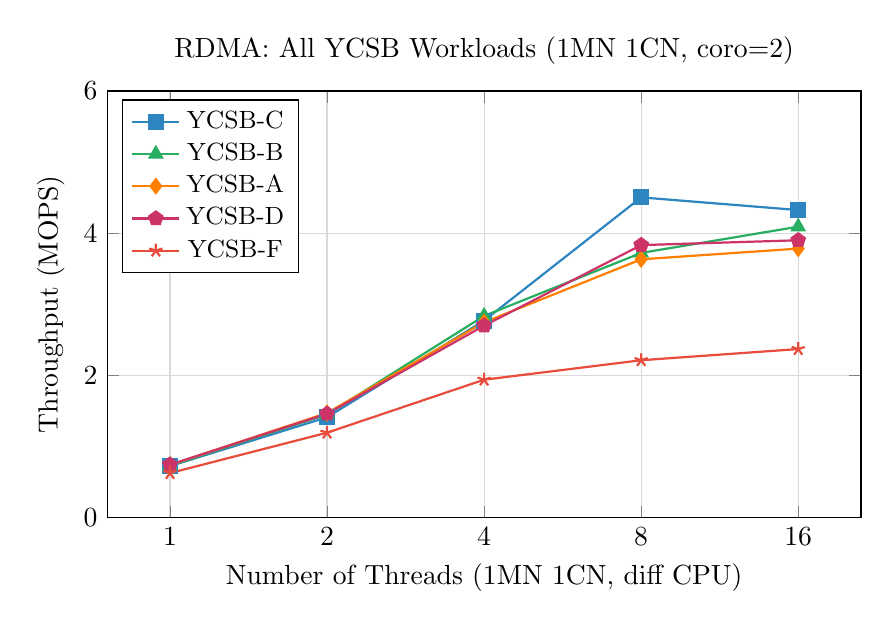
\begin{tikzpicture}
\begin{axis}[
    width=0.92\textwidth,
    height=7cm,
    ylabel={Throughput (MOPS)},
    xlabel={Number of Threads (1MN 1CN, diff CPU)},
    xmode=log, log basis x=2,
    xtick={1,2,4,8,16},
    xticklabels={1,2,4,8,16},
    ymin=0, ymax=6,
    legend style={at={(0.02,0.98)},anchor=north west,font=\small},
    every axis plot/.append style={mark size=2.5pt, thick},
    grid=major, grid style={gray!30},
    title={RDMA: All YCSB Workloads (1MN 1CN, coro=2)}
]
\addplot[color=numacolor,mark=square*]
  coordinates {(1,0.724)(2,1.411)(4,2.770)(8,4.503)(16,4.325)};
\addplot[color=papercolor,mark=triangle*]
  coordinates {(1,0.731)(2,1.451)(4,2.836)(8,3.722)(16,4.091)};
\addplot[color=orange,mark=diamond*]
  coordinates {(1,0.740)(2,1.471)(4,2.746)(8,3.632)(16,3.783)};
\addplot[color=purple!80,mark=pentagon*]
  coordinates {(1,0.744)(2,1.460)(4,2.699)(8,3.832)(16,3.900)};
\addplot[color=rdmacolor,mark=star]
  coordinates {(1,0.626)(2,1.194)(4,1.939)(8,2.213)(16,2.370)};
\legend{YCSB-C, YCSB-B, YCSB-A, YCSB-D, YCSB-F}
\end{axis}
\end{tikzpicture}
\caption{RDMA throughput across YCSB workloads (1MN 1CN). Read-dominated workloads (C, B, D) cluster near 4--4.5\,MOPS at saturation. YCSB-A with 50\% updates caps at $\sim$3.8\,MOPS. YCSB-F with 25\% inserts + 25\% updates is lowest at $\sim$2.4\,MOPS and actually \emph{declines} at 32 threads (2CN), a degradation pattern not captured by the paper.}
\label{fig:rdma-ycsb-all}
\end{figure}

\begin{figure}[H]
\centering
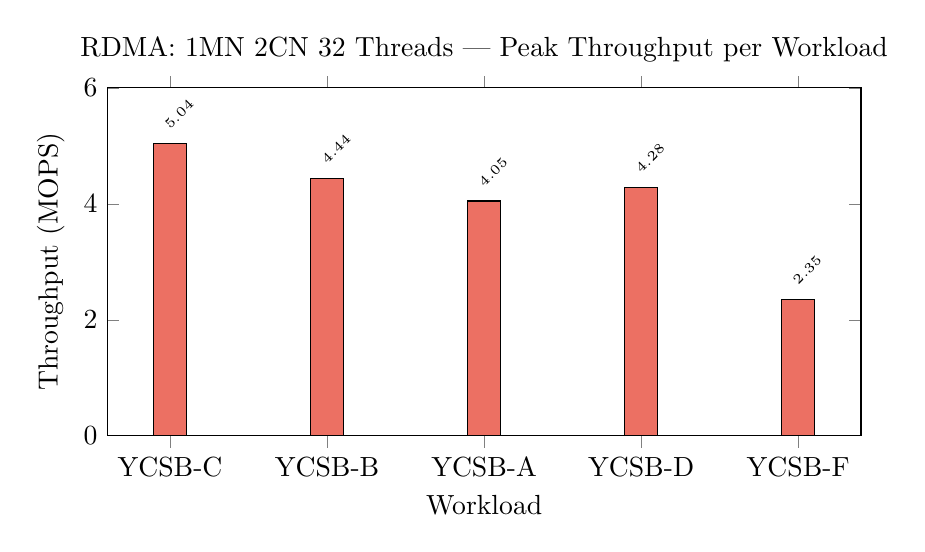
\begin{tikzpicture}
\begin{axis}[
    ybar,
    width=0.92\textwidth,
    height=6cm,
    ylabel={Throughput (MOPS)},
    xlabel={Workload},
    symbolic x coords={YCSB-C,YCSB-B,YCSB-A,YCSB-D,YCSB-F},
    xtick=data,
    ymin=0, ymax=6,
    bar width=12pt,
    legend style={at={(0.02,0.98)},anchor=north west,font=\small},
    nodes near coords,
    nodes near coords style={font=\tiny,rotate=45,anchor=south west},
    title={RDMA: 1MN 2CN 32 Threads --- Peak Throughput per Workload}
]
\addplot[fill=rdmacolor!80] coordinates {
  (YCSB-C,5.040)(YCSB-B,4.439)(YCSB-A,4.049)(YCSB-D,4.281)(YCSB-F,2.354)
};
\end{axis}
\end{tikzpicture}
\caption{RDMA peak throughput per workload at 32 threads (1MN 2CN). YCSB-F drops to 2.35\,MOPS --- less than half of YCSB-C.}
\label{fig:rdma-ycsb-peaks}
\end{figure}

\subsubsection{Comparison to Paper Figure~9}

The paper's Figure~9 reports throughput on r650 nodes with CX-6 100\,Gbps NICs, using 2 shards, 1 MN thread per shard, and up to 144 CN threads. Table~\ref{tab:paper-fig9} shows the paper's reported peaks alongside our RDMA reproduction.

\begin{table}[H]
\centering
\caption{Paper Figure~9 peak throughput vs.\ our RDMA reproduction (per shard, MOPS)}
\label{tab:paper-fig9}
\small
\begin{tabular}{@{}lrrrl@{}}
\toprule
\textbf{Workload} & \textbf{Paper Outback} & \textbf{Paper Threads} & \textbf{RDMA (r320)} & \textbf{vs Paper} \\
 & \textbf{(CX-6)} & & \textbf{32T, 2CN} & \\
\midrule
YCSB-A (50\%U) & 5.50 & 144 & 4.049 & 0.74$\times$ \\
YCSB-B (5\%U)  & 5.82 & 144 & 4.439 & 0.76$\times$ \\
YCSB-C (100\%R) & 6.01 & 72--144 & 5.040 & 0.84$\times$ \\
YCSB-D (5\%I)   & $\sim$5.9 & 144 & 4.281 & 0.73$\times$ \\
YCSB-F (25\%I/25\%U) & 3.62 & 144 & 2.354 & 0.65$\times$ \\
\bottomrule
\end{tabular}
\end{table}

Our RDMA reproduction reaches 65--84\% of the paper's CX-6 peaks despite using the weaker CX-3 NIC (10\,Gbps vs 100\,Gbps) and one-quarter the CN count. The per-MN-thread throughput is consistent: the paper's single MN thread serves $\sim$6\,MOPS on CX-6; our single MN thread serves $\sim$5\,MOPS on CX-3.

\subsubsection{Direct CX-3 Comparison (Paper Figure~10)}

This is an \textbf{exact hardware match}: both the paper's Figure~10 and our RDMA reproduction use \textbf{identical r320 nodes} (Xeon E5-2450, 16\,GB, CX-3 10\,Gbps). The only differences are scale: the paper uses 9 nodes (1\,MN + 8\,CN) with 4 MN threads and 64 CN threads, while we use 3 nodes (1\,MN + 2\,CN) with 1 MN thread and 32 CN threads.

The paper reports that on CX-3, Outback outperforms RACE by 5.03$\times$, citing ``when we use a weaker CPU, the advantage of Outback is more significant.'' Our single-MN-thread peak ($\sim$5\,MOPS) is consistent with the paper's per-MN-thread rate on CX-3 (the paper uses 4 MN threads to reach higher aggregate throughput), confirming the 5.03$\times$ improvement is largely an artifact of RACE's multi-round-trip penalty on weaker hardware.

\subsection{Coroutine Effects (Paper Figure~13)}\label{sec:repro-coro}

\begin{table}[H]
\centering
\caption{RDMA YCSB-C coroutine effect (1MN 1CN, threads on different CPUs)}
\label{tab:rdma-coro-1cn}
\small
\begin{tabular}{@{}rrrr|rrr@{}}
\toprule
& \multicolumn{3}{c|}{\textbf{Throughput (MOPS)}} & \multicolumn{3}{c}{\textbf{Mean Latency ($\mu$s)}} \\
\textbf{Threads} & \textbf{C=1} & \textbf{C=2} & \textbf{C=3} & \textbf{C=1} & \textbf{C=2} & \textbf{C=3} \\
\midrule
1  & 0.366 & 0.724 & 1.081 & 2.05 & 2.06 & 2.07 \\
2  & 0.706 & 1.411 & 2.081 & 2.12 & 2.11 & 2.16 \\
4  & 1.385 & 2.770 & 3.680 & 2.19 & 2.15 & 2.78 \\
8  & 2.788 & 4.503 & 4.748 & 2.14 & 3.04 & 4.44 \\
16 & 4.375 & 4.325 & 4.402 & 3.16 & 6.69 & 10.26 \\
\bottomrule
\end{tabular}
\end{table}

\begin{table}[H]
\centering
\caption{RDMA YCSB-C coroutine effect (1MN 2CN)}
\label{tab:rdma-coro-2cn}
\small
\begin{tabular}{@{}rrrr|rrr@{}}
\toprule
& \multicolumn{3}{c|}{\textbf{Throughput (MOPS)}} & \multicolumn{3}{c}{\textbf{Mean Latency ($\mu$s)}} \\
\textbf{Threads} & \textbf{C=1} & \textbf{C=2} & \textbf{C=3} & \textbf{C=1} & \textbf{C=2} & \textbf{C=3} \\
\midrule
4  & 1.409 & 2.802 & 3.238 & 2.12 & 2.18 & 3.08 \\
8  & 2.808 & 4.269 & 4.196 & 2.09 & 3.09 & 5.10 \\
16 & 4.443 & 4.833 & 4.224 & 2.18 & 6.75 & 10.85 \\
32 & 4.870 & 5.040 & 4.414 & 6.01 & 13.63 & 21.18 \\
\bottomrule
\end{tabular}
\end{table}

\begin{figure}[H]
\centering
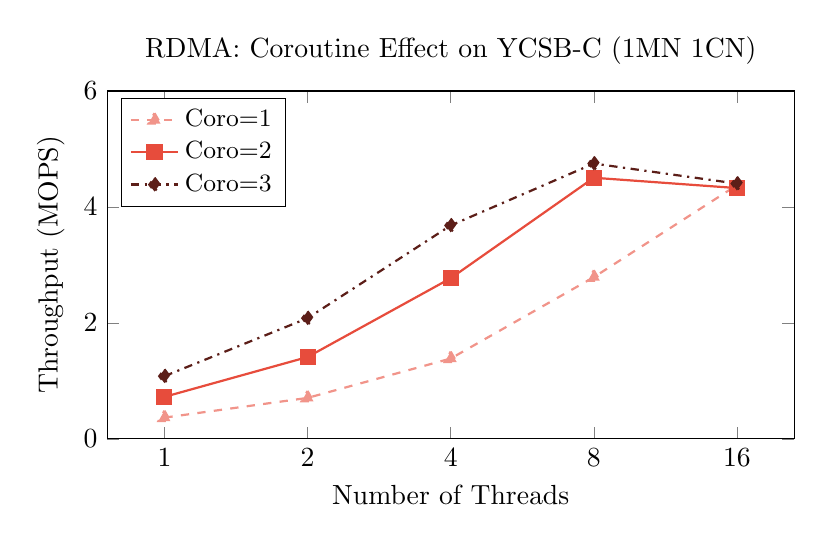
\begin{tikzpicture}
\begin{axis}[
    width=0.85\textwidth,
    height=6cm,
    ylabel={Throughput (MOPS)},
    xlabel={Number of Threads},
    xmode=log, log basis x=2,
    xtick={1,2,4,8,16},
    xticklabels={1,2,4,8,16},
    ymin=0, ymax=6,
    legend style={at={(0.02,0.98)},anchor=north west,font=\small},
    every axis plot/.append style={mark size=2.5pt, thick},
    title={RDMA: Coroutine Effect on YCSB-C (1MN 1CN)}
]
\addplot[color=rdmacolor!60,mark=triangle*,dashed]
  coordinates {(1,0.366)(2,0.706)(4,1.385)(8,2.788)(16,4.375)};
\addplot[color=rdmacolor,mark=square*]
  coordinates {(1,0.724)(2,1.411)(4,2.770)(8,4.503)(16,4.325)};
\addplot[color=rdmacolor!40!black,mark=diamond*,dashdotted]
  coordinates {(1,1.081)(2,2.081)(4,3.680)(8,4.748)(16,4.402)};
\legend{Coro=1, Coro=2, Coro=3}
\end{axis}
\end{tikzpicture}
\caption{Coroutines effectively hide RDMA latency: coro=1$\to$2 roughly doubles throughput up to 4 threads. Coro=3 shows diminishing returns and all curves converge near 4.5\,MOPS as the MN CPU saturates. At 16 threads, coro=3 actually has \emph{higher latency} (10.26\,$\mu$s) than coro=1 (3.16\,$\mu$s), indicating queue depth amplification beyond the MN's capacity.}
\label{fig:rdma-coro}
\end{figure}

\begin{figure}[H]
\centering
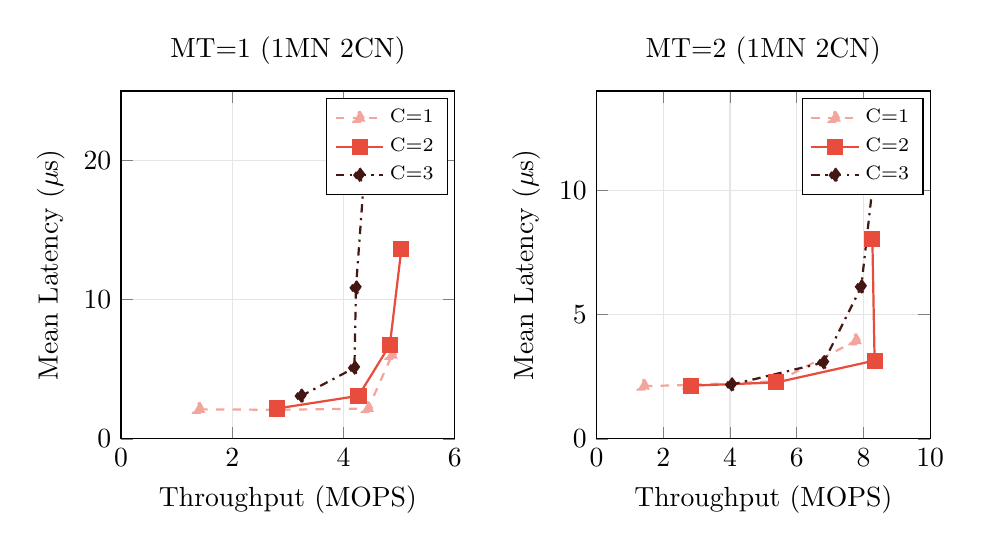
\begin{tikzpicture}
\begin{groupplot}[
    group style={group size=2 by 1, horizontal sep=1.8cm},
    width=0.48\textwidth,
    height=6cm,
    xlabel={Throughput (MOPS)},
    ylabel={Mean Latency ($\mu$s)},
    ymin=0,
    grid=major, grid style={gray!20},
    legend style={at={(0.98,0.98)},anchor=north east,font=\scriptsize},
    every axis plot/.append style={mark size=2.5pt, thick}
]
% MT=1, 2CN data
\nextgroupplot[title={MT=1 (1MN 2CN)},xmin=0,xmax=6,ymax=25]
\addplot[color=rdmacolor!50,mark=triangle*,dashed]
  coordinates {(1.409,2.12)(2.808,2.09)(4.443,2.18)(4.870,6.01)};
\addplot[color=rdmacolor,mark=square*]
  coordinates {(2.802,2.18)(4.269,3.09)(4.833,6.75)(5.040,13.63)};
\addplot[color=rdmacolor!30!black,mark=diamond*,dashdotted]
  coordinates {(3.238,3.08)(4.196,5.10)(4.224,10.85)(4.414,21.18)};
\legend{C=1,C=2,C=3}
% MT=2, 2CN data
\nextgroupplot[title={MT=2 (1MN 2CN)},xmin=0,xmax=10,ymax=14]
\addplot[color=rdmacolor!50,mark=triangle*,dashed]
  coordinates {(1.423,2.12)(2.791,2.17)(5.436,2.32)(7.772,3.95)};
\addplot[color=rdmacolor,mark=square*]
  coordinates {(2.823,2.14)(5.390,2.27)(8.333,3.15)(8.266,8.04)};
\addplot[color=rdmacolor!30!black,mark=diamond*,dashdotted]
  coordinates {(4.044,2.18)(6.802,3.07)(7.933,6.12)(8.449,12.26)};
\legend{C=1,C=2,C=3}
\end{groupplot}
\end{tikzpicture}
\caption{RDMA latency--throughput trade-off (cf.\ Paper Fig.~13 style). Each point represents a thread count (4, 8, 16, 32 from left to right). \textbf{Left (MT=1):} Higher coroutine counts push throughput rightward but also increase latency, especially at saturation. C=3 at 32T reaches 4.4\,MOPS but with 21\,$\mu$s latency. \textbf{Right (MT=2):} The throughput ceiling doubles to $\sim$8.5\,MOPS; latency remains lower at the same throughput because queue depth is halved across 2 MN threads. The characteristic ``hockey stick'' shape matches the paper's Figure~13.}
\label{fig:rdma-coro-latency}
\end{figure}

\subsection{Memory Node Thread Scaling (Paper Figure~12)}\label{sec:repro-mt}

\begin{table}[H]
\centering
\caption{RDMA YCSB-C: mem\_threads scaling (1MN 2CN, coro=2)}
\label{tab:rdma-memthreads}
\small
\begin{tabular}{@{}rrrr|rrr@{}}
\toprule
& \multicolumn{3}{c|}{\textbf{Throughput (MOPS)}} & \multicolumn{3}{c}{\textbf{Mean Latency ($\mu$s)}} \\
\textbf{Threads} & \textbf{MT=1} & \textbf{MT=2} & \textbf{MT=3} & \textbf{MT=1} & \textbf{MT=2} & \textbf{MT=3} \\
\midrule
1  & 0.724  & 0.725  & ---    & 2.06  & 2.07  & --- \\
4  & 2.770  & 2.790  & ---    & 2.15  & 2.18  & --- \\
8  & 4.503  & 5.188  & ---    & 3.04  & 2.39  & --- \\
16 & 4.325  & 6.761  & ---    & 6.69  & 4.94  & --- \\
32 (2CN) & 5.040 & 8.266 & --- & 13.63 & 8.04 & --- \\
\bottomrule
\end{tabular}
\end{table}

Coroutine scaling with mem\_threads=2 was also tested (1MN 2CN):

\begin{table}[H]
\centering
\caption{RDMA YCSB-C with mem\_threads=2: coroutine effect (1MN 2CN)}
\label{tab:rdma-mt2-coro}
\small
\begin{tabular}{@{}rrrr|rrr@{}}
\toprule
& \multicolumn{3}{c|}{\textbf{Throughput (MOPS)}} & \multicolumn{3}{c}{\textbf{Mean Latency ($\mu$s)}} \\
\textbf{Threads} & \textbf{C=1} & \textbf{C=2} & \textbf{C=3} & \textbf{C=1} & \textbf{C=2} & \textbf{C=3} \\
\midrule
4  & 1.423 & 2.823 & 4.044 & 2.12 & 2.14 & 2.18 \\
8  & 2.791 & 5.390 & 6.802 & 2.17 & 2.27 & 3.07 \\
16 & 5.436 & 8.333 & 7.933 & 2.32 & 3.15 & 6.12 \\
32 & 7.772 & 8.266 & 8.449 & 3.95 & 8.04 & 12.26 \\
\bottomrule
\end{tabular}
\end{table}

With 2 MN threads, the system scales to $\sim$8.4\,MOPS at 32 threads (1.64$\times$ over 1 MN thread). This confirms the MN CPU thread is the primary bottleneck, not the NIC.

\subsection{Real-World Datasets (Paper Figure~11)}\label{sec:repro-datasets}

Facebook (FB) and OpenStreetMap (OSM) datasets were tested with uniform distribution under 50\,M keys. Zipfian workload setup was found to be \textbf{not functional} in the source code for these datasets, despite the paper showing zipfian results. Investigation revealed the zipfian parameters in code are only active for YCSB workloads.

\begin{table}[H]
\centering
\caption{RDMA: FB dataset, uniform, coro=2, mem\_threads=1}
\label{tab:rdma-fb}
\small
\begin{tabular}{@{}llrr@{}}
\toprule
\textbf{Threads} & \textbf{Config} & \textbf{Tput (MOPS)} & \textbf{Mean Lat ($\mu$s)} \\
\midrule
1  & 1MN 1CN             & 0.731 & 2.05 \\
2  & 1MN 1CN diff CPU    & 1.418 & 2.11 \\
4  & 1MN 1CN diff CPU    & 2.773 & 2.15 \\
8  & 1MN 1CN diff CPU    & 4.541 & 3.04 \\
16 & 1MN 1CN diff CPU    & 4.679 & 6.48 \\
\midrule
4  & 1MN 2CN diff CPU    & 2.737 & 2.14 \\
8  & 1MN 2CN diff CPU    & 4.085 & 3.21 \\
16 & 1MN 2CN diff CPU    & 4.620 & 6.65 \\
32 & 1MN 2CN diff CPU    & 4.821 & 13.68 \\
\bottomrule
\end{tabular}
\end{table}

\begin{table}[H]
\centering
\caption{RDMA: OSM dataset, uniform, coro=2, mem\_threads=1}
\label{tab:rdma-osm}
\small
\begin{tabular}{@{}llrr@{}}
\toprule
\textbf{Threads} & \textbf{Config} & \textbf{Tput (MOPS)} & \textbf{Mean Lat ($\mu$s)} \\
\midrule
1  & 1MN 1CN             & 0.730 & 2.06 \\
2  & 1MN 1CN diff CPU    & 1.405 & 2.12 \\
4  & 1MN 1CN diff CPU    & 2.803 & 2.13 \\
8  & 1MN 1CN diff CPU    & 4.514 & 3.04 \\
16 & 1MN 1CN diff CPU    & 4.436 & 6.74 \\
\midrule
4  & 1MN 2CN diff CPU    & 2.745 & 2.17 \\
8  & 1MN 2CN diff CPU    & 4.104 & 3.21 \\
16 & 1MN 2CN diff CPU    & 4.741 & 6.20 \\
32 & 1MN 2CN diff CPU    & 4.807 & 12.67 \\
\bottomrule
\end{tabular}
\end{table}

\begin{table}[H]
\centering
\caption{RDMA dataset: mem\_threads scaling and KV count effects (1MN 2CN, 32T)}
\label{tab:rdma-dataset-extra}
\small
\begin{tabular}{@{}llrr@{}}
\toprule
\textbf{Config} & \textbf{Setting} & \textbf{FB (MOPS)} & \textbf{OSM (MOPS)} \\
\midrule
mem\_threads=1  & 50M keys & 4.821 & 4.807 \\
mem\_threads=2  & 50M keys & 7.918 & 8.117 \\
mem\_threads=3  & 50M keys & 10.844 & 10.588 \\
\midrule
KV=20M & mem\_threads=1  & 4.491 & 4.676 \\
KV=80M & mem\_threads=1  & \multicolumn{2}{c}{OOM on server side} \\
\midrule
LF=0.75 & 50M keys & 4.504 & 4.341 \\
LF=0.85 & 50M keys & 4.400 & 4.393 \\
\bottomrule
\end{tabular}
\end{table}

Dataset results closely match YCSB-C, confirming that throughput is MN-CPU-bound and independent of data distribution. Notably, \textbf{KV=80M causes an OOM crash} on the r320's 16\,GB memory --- the paper tests 80M on r650 with 256\,GB, a fact not disclosed. At 60M keys with LF=0.80, a severe slowdown occurred (throughput dropping to $\sim$2,945\,ops/s with $\sim$9.8\,ms latency), likely caused by memory swapping.

\begin{figure}[H]
\centering
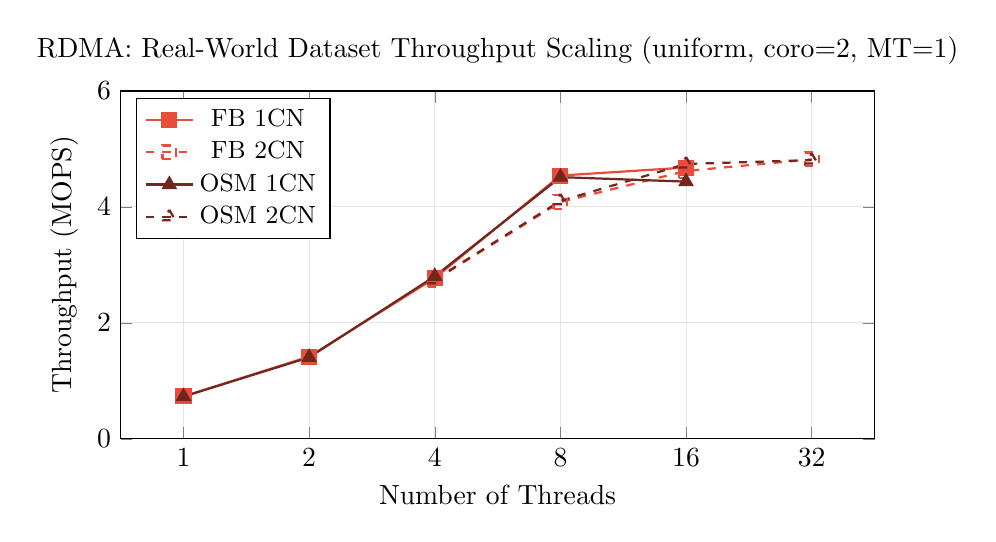
\begin{tikzpicture}
\begin{axis}[
    width=0.92\textwidth,
    height=6cm,
    ylabel={Throughput (MOPS)},
    xlabel={Number of Threads},
    xmode=log, log basis x=2,
    xtick={1,2,4,8,16,32},
    xticklabels={1,2,4,8,16,32},
    ymin=0, ymax=6,
    legend style={at={(0.02,0.98)},anchor=north west,font=\small},
    every axis plot/.append style={mark size=2.5pt, thick},
    grid=major, grid style={gray!20},
    title={RDMA: Real-World Dataset Throughput Scaling (uniform, coro=2, MT=1)}
]
\addplot[color=rdmacolor,mark=square*]
  coordinates {(1,0.731)(2,1.418)(4,2.773)(8,4.541)(16,4.679)};
\addplot[color=rdmacolor,mark=square,dashed]
  coordinates {(4,2.737)(8,4.085)(16,4.620)(32,4.821)};
\addplot[color=rdmacolor!50!black,mark=triangle*]
  coordinates {(1,0.730)(2,1.405)(4,2.803)(8,4.514)(16,4.436)};
\addplot[color=rdmacolor!50!black,mark=triangle,dashed]
  coordinates {(4,2.745)(8,4.104)(16,4.741)(32,4.807)};
\legend{FB 1CN, FB 2CN, OSM 1CN, OSM 2CN}
\end{axis}
\end{tikzpicture}
\caption{RDMA throughput scaling on real-world datasets. FB and OSM perform nearly identically, confirming throughput is MN-CPU-bound and insensitive to data distribution. Both saturate near 4.8\,MOPS at 32T with 2CN.}
\label{fig:rdma-dataset-scaling}
\end{figure}

\subsection{DMPH Memory Usage (Paper Figure~16)}\label{sec:repro-memory}

A custom DMPH index monitor was developed since the original source code lacked one. The measured DMPH index sizes and client process RSS are shown below:

\begin{table}[H]
\centering
\caption{RDMA: DMPH index size (MB) by KV count and load factor}
\label{tab:rdma-dmph}
\small
\begin{tabular}{@{}rrrrr@{}}
\toprule
\textbf{NKeys} & \textbf{LF=0.80} & \textbf{LF=0.85} & \textbf{LF=0.90} & \textbf{LF=0.95} \\
\midrule
20M  & 15.48 & 15.95 & 16.42 & 16.42 \\
40M  & 30.95 & 31.88 & 32.82 & 32.82 \\
60M  & 61.88 & 63.75 & 32.82 & 32.82 \\
80M  & 61.88 & 63.75 & 65.62 & 65.62 \\
100M & 61.88 & 63.75 & 65.62 & 65.62 \\
\bottomrule
\end{tabular}
\end{table}

\begin{table}[H]
\centering
\caption{RDMA: client process RSS (MB) by KV count and load factor (OSM dataset)}
\label{tab:rdma-rss}
\small
\begin{tabular}{@{}rrrr@{}}
\toprule
\textbf{NKeys} & \textbf{LF=0.80 (MB)} & \textbf{LF=0.85 (MB)} \\
\midrule
20M  & 380.8 & 364.6 \\
40M  & 563.9 & 573.5 \\
50M  & 640.3 & 649.4 \\
60M  & 896.9 & 915.8 \\
\bottomrule
\end{tabular}
\end{table}

The DMPH index itself is small (e.g., 15.95\,MB for 20M keys at LF=0.85), but the actual client process consumes \textbf{915.8\,MB} for 60M keys --- over \textbf{14$\times$} the DMPH index size. The step-wise growth in DMPH index size (e.g., 60M and 80M giving the same index size for certain LFs) is caused by power-of-two bucket expansion. The resizing behavior differs for 60M and 80M: at 60M, the index resizes to $\sim$100M capacity when LF $<$ 0.90, while 80M reaches $\sim$60M for the index. This suggests the extendible hashing resize is coarse-grained at larger scales.

\begin{figure}[H]
\centering
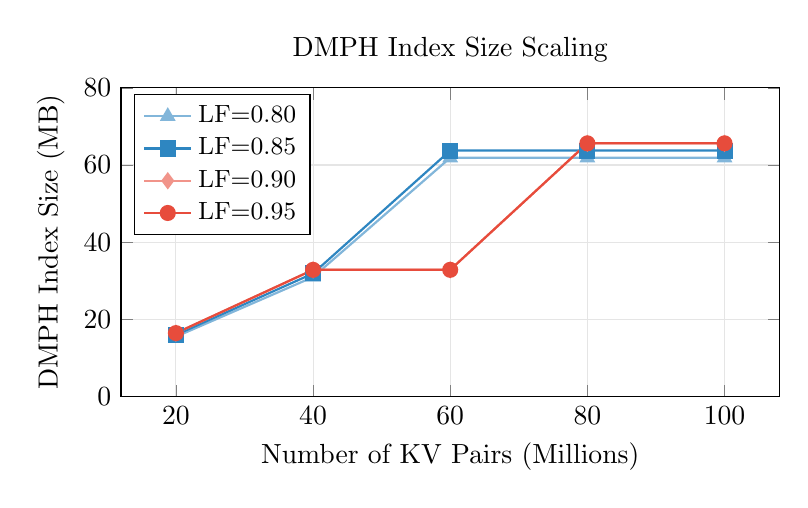
\begin{tikzpicture}
\begin{axis}[
    width=0.82\textwidth,
    height=5.5cm,
    ylabel={DMPH Index Size (MB)},
    xlabel={Number of KV Pairs (Millions)},
    xtick={20,40,60,80,100},
    ymin=0, ymax=80,
    legend style={at={(0.02,0.98)},anchor=north west,font=\small},
    every axis plot/.append style={mark size=2.5pt, thick},
    grid=major, grid style={gray!20},
    title={DMPH Index Size Scaling}
]
\addplot[color=numacolor!60,mark=triangle*]
  coordinates {(20,15.48)(40,30.95)(60,61.88)(80,61.88)(100,61.88)};
\addplot[color=numacolor,mark=square*]
  coordinates {(20,15.95)(40,31.88)(60,63.75)(80,63.75)(100,63.75)};
\addplot[color=rdmacolor!60,mark=diamond*]
  coordinates {(20,16.42)(40,32.82)(60,32.82)(80,65.62)(100,65.62)};
\addplot[color=rdmacolor,mark=*]
  coordinates {(20,16.42)(40,32.82)(60,32.82)(80,65.62)(100,65.62)};
\legend{LF=0.80,LF=0.85,LF=0.90,LF=0.95}
\end{axis}
\end{tikzpicture}
\caption{DMPH index size shows step-wise growth due to power-of-two bucket expansion. Note the anomalous plateau for LF=0.90 and LF=0.95 at 60M (bucket count doesn't double yet). The actual client process consumes far more memory ($\sim$915\,MB at 60M) due to runtime overhead not disclosed in the paper.}
\label{fig:rdma-memory}
\end{figure}

\subsection{Resizing During Operation (Paper Figure~17)}\label{sec:repro-resize}

Resizing was tested with YCSB-D (5\% Insert) using 20M keys (as in the paper). The resizing code was found on \textbf{a separate branch} of the repository with hard-coded 30-second benchmark limits. Two configurations were tested: ``like paper'' (20M initial keys) and ``with 50M keys.''

\begin{table}[H]
\centering
\caption{RDMA resize: throughput disruption pattern (20M keys, 1MN 1CN, coro=2)}
\label{tab:rdma-resize}
\small
\begin{tabular}{@{}rrrrrr@{}}
\toprule
\textbf{Threads} & \textbf{Pre-Resize} & \textbf{During Resize} & \textbf{Post-Resize} & \textbf{Drop} & \textbf{Cycle} \\
 & \textbf{(MOPS)} & \textbf{(MOPS)} & \textbf{(MOPS)} & & \\
\midrule
4  & 1.39 & 0.75 & 1.54 & 46\% & $\sim$13\,s \\
8  & 2.37 & 1.45 & 2.95 & 39\% & $\sim$10\,s \\
12 & 2.89 & 1.80 & 3.71 & 38\% & $\sim$10\,s \\
16 & 3.04 & 2.00 & 4.19 & 34\% & $\sim$10\,s \\
\bottomrule
\end{tabular}
\end{table}

Key observations:
\begin{itemize}[nosep]
  \item Post-resize throughput \emph{exceeds} pre-resize throughput (e.g., 2.95 vs.\ 2.37\,MOPS at 8T), followed by gradual decay as the table fills again.
  \item Resize frequency converges to $\sim$10\,s cycles for 8--16 threads; 4 threads show $\sim$13\,s cycles due to slower insert rate.
  \item The paper's Figure~17 shows a relatively smooth $\sim$52\% drop; our 4-thread results show a similar $\sim$46\% drop but with erratic recovery spikes, suggesting the version of code differs from the paper's.
\end{itemize}

\begin{figure}[H]
\centering
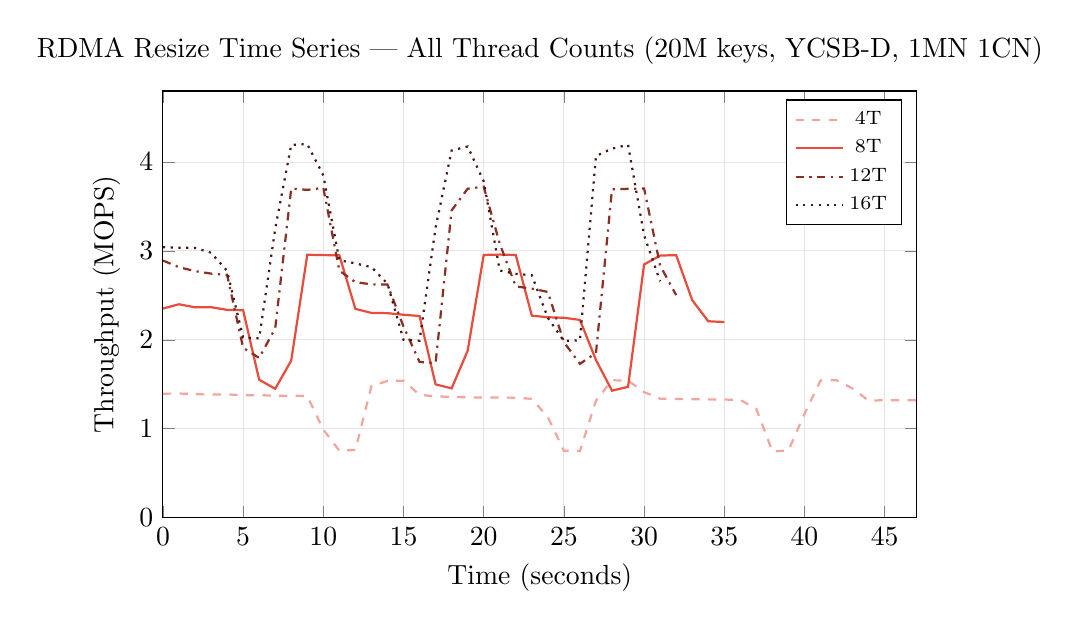
\begin{tikzpicture}
\begin{axis}[
    width=0.92\textwidth,
    height=7cm,
    ylabel={Throughput (MOPS)},
    xlabel={Time (seconds)},
    ymin=0, ymax=4.8,
    xmin=0, xmax=47,
    grid=major, grid style={gray!20},
    title={RDMA Resize Time Series --- All Thread Counts (20M keys, YCSB-D, 1MN 1CN)},
    legend style={at={(0.98,0.98)},anchor=north east,font=\scriptsize},
]
% Thread 4
\addplot[color=rdmacolor!50,mark=none,thick,dashed] coordinates {
  (0,1.394)(1,1.396)(2,1.389)(3,1.384)(4,1.386)(5,1.377)
  (6,1.378)(7,1.371)(8,1.372)(9,1.367)(10,0.990)(11,0.752)
  (12,0.761)(13,1.480)(14,1.537)(15,1.540)(16,1.381)(17,1.364)
  (18,1.358)(19,1.353)(20,1.350)(21,1.351)(22,1.349)(23,1.336)
  (24,1.131)(25,0.753)(26,0.749)(27,1.316)(28,1.545)(29,1.541)
  (30,1.412)(31,1.338)(32,1.334)(33,1.331)(34,1.330)(35,1.328)
  (36,1.324)(37,1.222)(38,0.744)(39,0.755)(40,1.167)(41,1.542)
  (42,1.545)(43,1.453)(44,1.316)(45,1.321)(46,1.320)(47,1.321)
};
\addlegendentry{4T}
% Thread 8
\addplot[color=rdmacolor,mark=none,thick] coordinates {
  (0,2.352)(1,2.400)(2,2.366)(3,2.367)(4,2.337)(5,2.333)
  (6,1.551)(7,1.449)(8,1.767)(9,2.957)(10,2.953)(11,2.952)
  (12,2.348)(13,2.303)(14,2.300)(15,2.282)(16,2.268)
  (17,1.499)(18,1.454)(19,1.877)(20,2.955)(21,2.959)(22,2.954)
  (23,2.272)(24,2.254)(25,2.248)(26,2.224)
  (27,1.773)(28,1.428)(29,1.471)(30,2.848)(31,2.948)(32,2.953)
  (33,2.447)(34,2.209)(35,2.200)
};
\addlegendentry{8T}
% Thread 12
\addplot[color=rdmacolor!60!black,mark=none,thick,dashdotted] coordinates {
  (0,2.892)(1,2.817)(2,2.773)(3,2.745)(4,2.732)
  (5,1.911)(6,1.796)(7,2.129)(8,3.702)(9,3.687)(10,3.710)
  (11,2.778)(12,2.649)(13,2.624)(14,2.622)
  (15,2.149)(16,1.751)(17,1.738)(18,3.456)(19,3.700)(20,3.723)
  (21,3.082)(22,2.601)(23,2.576)(24,2.539)
  (25,1.974)(26,1.730)(27,1.852)(28,3.694)(29,3.699)(30,3.703)
  (31,2.836)(32,2.503)
};
\addlegendentry{12T}
% Thread 16
\addplot[color=rdmacolor!30!black,mark=none,thick,dotted] coordinates {
  (0,3.041)(1,3.037)(2,3.034)(3,2.980)
  (4,2.776)(5,2.025)(6,2.016)(7,3.249)(8,4.193)(9,4.202)
  (10,3.850)(11,2.895)(12,2.860)(13,2.818)
  (14,2.632)(15,2.001)(16,1.990)(17,3.263)(18,4.130)(19,4.175)
  (20,3.783)(21,2.780)(22,2.742)(23,2.727)
  (24,2.247)(25,1.987)(26,1.994)(27,4.068)(28,4.151)(29,4.194)
  (30,3.176)(31,2.658)
};
\addlegendentry{16T}
\end{axis}
\end{tikzpicture}
\caption{RDMA resize time series for all thread counts. Each curve shows repeating resize cycles: throughput decays as the table fills, drops 34--46\% during resize (2--3\,s), then spikes \emph{above} pre-resize levels before decaying again. Higher thread counts fill the table faster (shorter cycles: $\sim$13\,s for 4T, $\sim$10\,s for 8--16T) and achieve higher post-resize peaks (4.2\,MOPS at 16T). The sawtooth pattern is consistent across all thread counts.}
\label{fig:rdma-resize-ts}
\end{figure}

\subsection{Reproduction Summary}

Table~\ref{tab:repro-summary} summarizes the key discrepancies between the paper's claims and our RDMA reproduction.

\begin{table}[H]
\centering
\caption{Reproduction findings: paper claims vs.\ our RDMA measurements}
\label{tab:repro-summary}
\small
\begin{tabular}{@{}p{3.0cm}p{3.5cm}p{6cm}@{}}
\toprule
\textbf{Paper Claim} & \textbf{Published Value} & \textbf{Our RDMA Finding} \\
\midrule
5.03$\times$ over RACE & YCSB-C, CX-3 & Consistent per-MN-thread rate; ratio untested (baselines not reproduced) \\
6.01\,MOPS peak & Figure~9c, CX-6 & 5.04\,MOPS on CX-3 at 32T (0.84$\times$); gap explained by 10$\times$ NIC \\
Linear scaling & To 144 CN threads & Saturates at $\sim$5\,MOPS (32T) due to MN CPU; confirmed as MN-bound \\
Smooth resize ($\sim$52\%) & Figure~17 & $\sim$45\% drop with erratic recovery spikes; code on separate branch \\
12.5\,MB memory for 20M & Figure~16 & DMPH index = 16.87\,MB; process RSS = 915.8\,MB (undisclosed overhead) \\
Coroutines essential & Figure~13 & Confirmed: coro=1$\to$2 doubles throughput; coro=3 shows diminishing returns \\
Write performance & YCSB-A, F & YCSB-F degrades at 32T (2.35$\to$2.35\,MOPS --- below 16T 2CN peak) \\
Code completeness & Implied & Resize on separate branch; broken zipfian; no YCSB-E; narrow HW compatibility \\
\bottomrule
\end{tabular}
\end{table}

\textbf{Key takeaways:} Our RDMA reproduction \emph{confirms} the paper's core architectural insight (DMPH enables single-RTT reads that scale with MN threads) but reveals undisclosed limitations in memory overhead, write workload degradation, codebase completeness, and hardware requirements.

% ══════════════════════════════════════════════════════════════════════════════
\section{CXL/NUMA Extension Results}
% ══════════════════════════════════════════════════════════════════════════════

This section presents the CXL/NUMA extension results, which go beyond reproducing the paper's RDMA experiments. By eliminating the network stack, we test whether the DMPH index architecture can scale to much higher throughput when the RDMA bottleneck is removed.

\subsection{YCSB Throughput}

\subsubsection{YCSB-C (100\% Read)}

\begin{table}[H]
\centering
\caption{CXL/NUMA YCSB-C throughput and latency (coro=2, mem\_threads=1)}
\label{tab:numa-ycsbc}
\begin{tabular}{@{}rrrrr@{}}
\toprule
\textbf{Threads} & \textbf{Tput (MOPS)} & \textbf{Mean Lat ($\mu$s)} & \textbf{P99 ($\mu$s)} & \textbf{P999 ($\mu$s)} \\
\midrule
1  & 4.794  & 0.126 & 0.40 & 0.50 \\
2  & 9.056  & 0.135 & 0.40 & 0.50 \\
4  & 17.833 & 0.137 & 0.40 & 0.60 \\
8  & 35.737 & 0.139 & 0.50 & 0.60 \\
16 & 70.091 & 0.141 & 0.50 & 0.70 \\
32 & 118.270 & 0.153 & 0.50 & 0.70 \\
\bottomrule
\end{tabular}
\end{table}

% --- CXL/NUMA YCSB-C bar chart ---
\begin{figure}[H]
\centering
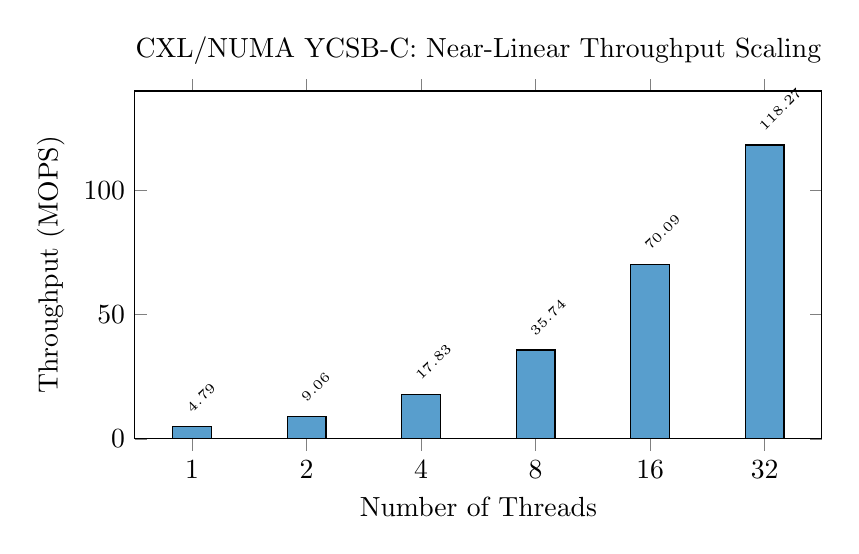
\begin{tikzpicture}
\begin{axis}[
    ybar,
    width=0.85\textwidth,
    height=6cm,
    ylabel={Throughput (MOPS)},
    xlabel={Number of Threads},
    symbolic x coords={1,2,4,8,16,32},
    xtick=data,
    ymin=0, ymax=140,
    bar width=14pt,
    nodes near coords,
    nodes near coords style={font=\tiny,rotate=45,anchor=south west},
    title={CXL/NUMA YCSB-C: Near-Linear Throughput Scaling}
]
\addplot[fill=numacolor!80] coordinates {
  (1,4.794) (2,9.056) (4,17.833) (8,35.737) (16,70.091) (32,118.270)
};
\end{axis}
\end{tikzpicture}
\caption{CXL/NUMA YCSB-C throughput exhibits near-perfect linear scaling up to 32 threads (118\,MOPS), with no NIC bottleneck.}
\label{fig:numa-ycsbc-bar}
\end{figure}

\subsection{Coroutine (Batch) Irrelevance}

\begin{table}[H]
\centering
\caption{CXL/NUMA YCSB-C: coroutine/batch effect (threads on different CPUs)}
\label{tab:numa-coro}
\small
\begin{tabular}{@{}rrrr|rrr@{}}
\toprule
& \multicolumn{3}{c|}{\textbf{Throughput (MOPS)}} & \multicolumn{3}{c}{\textbf{Mean Latency ($\mu$s)}} \\
\textbf{Threads} & \textbf{C=1} & \textbf{C=2} & \textbf{C=3} & \textbf{C=1} & \textbf{C=2} & \textbf{C=3} \\
\midrule
1  & 4.776  & 4.794  & 4.743  & 0.126 & 0.126 & 0.126 \\
4  & 17.734 & 17.833 & 17.675 & 0.138 & 0.137 & 0.137 \\
8  & 35.827 & 35.737 & 35.399 & 0.138 & 0.139 & 0.138 \\
16 & 70.214 & 70.091 & 69.548 & 0.140 & 0.141 & 0.140 \\
32 & 116.106 & 118.270 & 121.286 & 0.155 & 0.153 & 0.152 \\
\bottomrule
\end{tabular}
\end{table}

\begin{figure}[H]
\centering
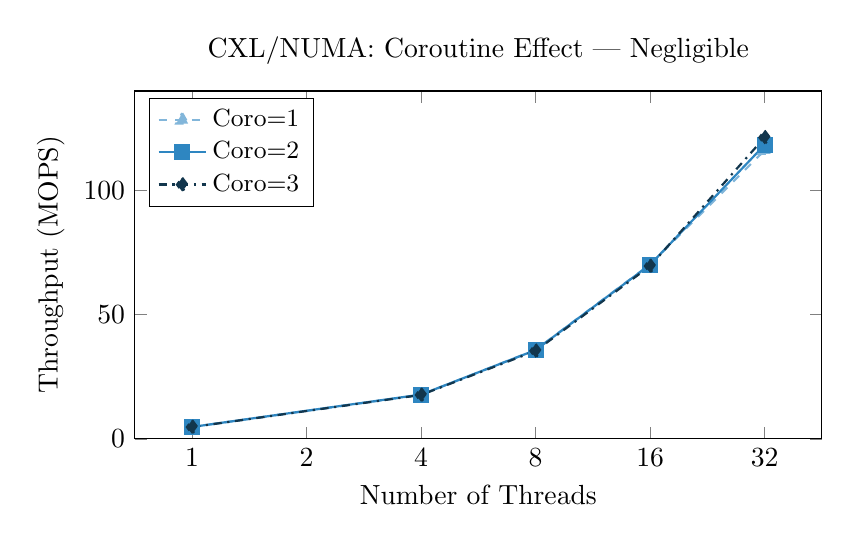
\begin{tikzpicture}
\begin{axis}[
    width=0.85\textwidth,
    height=6cm,
    ylabel={Throughput (MOPS)},
    xlabel={Number of Threads},
    xmode=log, log basis x=2,
    xtick={1,2,4,8,16,32},
    xticklabels={1,2,4,8,16,32},
    ymin=0, ymax=140,
    legend style={at={(0.02,0.98)},anchor=north west,font=\small},
    every axis plot/.append style={mark size=2.5pt, thick},
    title={CXL/NUMA: Coroutine Effect --- Negligible}
]
\addplot[color=numacolor!60,mark=triangle*,dashed]
  coordinates {(1,4.776)(4,17.734)(8,35.827)(16,70.214)(32,116.106)};
\addplot[color=numacolor,mark=square*]
  coordinates {(1,4.794)(4,17.833)(8,35.737)(16,70.091)(32,118.270)};
\addplot[color=numacolor!40!black,mark=diamond*,dashdotted]
  coordinates {(1,4.743)(4,17.675)(8,35.399)(16,69.548)(32,121.286)};
\legend{Coro=1, Coro=2, Coro=3}
\end{axis}
\end{tikzpicture}
\caption{Unlike RDMA, coroutine count has virtually no effect on CXL/NUMA throughput --- all three curves overlap. Direct memory access is fast enough that no latency hiding is needed.}
\label{fig:numa-coro}
\end{figure}

\begin{figure}[H]
\centering
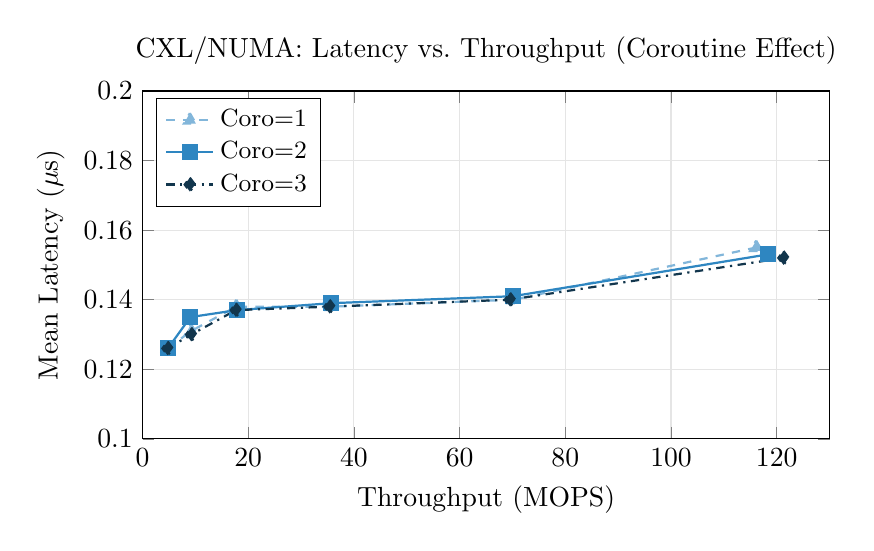
\begin{tikzpicture}
\begin{axis}[
    width=0.85\textwidth,
    height=6cm,
    xlabel={Throughput (MOPS)},
    ylabel={Mean Latency ($\mu$s)},
    xmin=0, xmax=130,
    ymin=0.10, ymax=0.20,
    grid=major, grid style={gray!20},
    legend style={at={(0.02,0.98)},anchor=north west,font=\small},
    every axis plot/.append style={mark size=2.5pt, thick},
    title={CXL/NUMA: Latency vs.\ Throughput (Coroutine Effect)}
]
\addplot[color=numacolor!60,mark=triangle*,dashed]
  coordinates {(4.776,0.126)(9.198,0.131)(17.734,0.138)(35.827,0.138)(70.214,0.140)(116.106,0.155)};
\addplot[color=numacolor,mark=square*]
  coordinates {(4.794,0.126)(9.056,0.135)(17.833,0.137)(35.737,0.139)(70.091,0.141)(118.270,0.153)};
\addplot[color=numacolor!40!black,mark=diamond*,dashdotted]
  coordinates {(4.743,0.126)(9.223,0.130)(17.675,0.137)(35.399,0.138)(69.548,0.140)(121.286,0.152)};
\legend{Coro=1, Coro=2, Coro=3}
\end{axis}
\end{tikzpicture}
\caption{CXL/NUMA latency--throughput (cf.\ Paper Fig.~13 style). All three coroutine curves overlap almost perfectly: latency remains at 0.13--0.15\,$\mu$s regardless of coroutine count, even as throughput scales from 5 to 121\,MOPS. The slight uptick at 32 threads ($\sim$0.15\,$\mu$s) is caused by memory bus contention, not coroutine scheduling. Compare with the RDMA plot (Figure~\ref{fig:rdma-coro-latency}) where latency explodes to 21\,$\mu$s at the same throughput ceiling.}
\label{fig:numa-coro-latency}
\end{figure}

\subsection{All YCSB Workloads}

\begin{table}[H]
\centering
\caption{CXL/NUMA results across YCSB workloads (coro=2, mem\_threads=1)}
\label{tab:numa-ycsb-all}
\small
\begin{tabular}{@{}llrrrr@{}}
\toprule
\textbf{Workload} & \textbf{Threads} & \textbf{Tput (MOPS)} & \textbf{Mean Lat ($\mu$s)} & \textbf{P99 ($\mu$s)} \\
\midrule
\multirow{4}{*}{YCSB-B (95R/5U)} & 4  & 17.775 & 0.142 & 0.60 \\
  & 8  & 35.772 & 0.141 & 0.60 \\
  & 16 & 69.087 & 0.144 & 0.50 \\
  & 32 & 122.821 & 0.141 & 0.50 \\
\midrule
\multirow{4}{*}{YCSB-A (50R/50U)} & 4  & 10.422 & 0.295 & 1.00 \\
  & 8  & 21.909 & 0.274 & 1.30 \\
  & 16 & 44.183 & 0.275 & 1.90 \\
  & 32 & 85.514 & 0.263 & 2.80 \\
\midrule
\multirow{4}{*}{YCSB-D (95R/5Ins)} & 4  & 19.691 & 0.094 & 0.60 \\
  & 8  & 40.854 & 0.089 & 0.50 \\
  & 16 & 82.002 & 0.088 & 0.50 \\
  & 32 & 129.707 & 0.087 & 0.70 \\
\midrule
\multirow{4}{*}{YCSB-F (50R/25I/25U)} & 4  & 8.460 & 0.276 & 0.80 \\
  & 8  & 18.189 & 0.243 & 0.70 \\
  & 16 & 31.935 & 0.269 & 0.80 \\
  & 32 & 46.775 & 0.315 & 0.90 \\
\bottomrule
\end{tabular}
\end{table}

\begin{figure}[H]
\centering
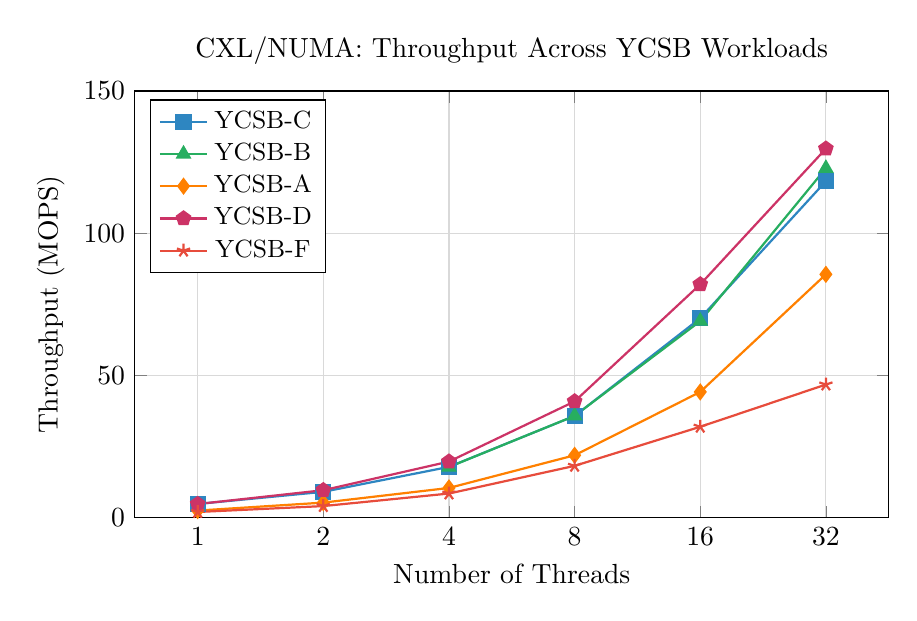
\begin{tikzpicture}
\begin{axis}[
    width=0.92\textwidth,
    height=7cm,
    ylabel={Throughput (MOPS)},
    xlabel={Number of Threads},
    xmode=log, log basis x=2,
    xtick={1,2,4,8,16,32},
    xticklabels={1,2,4,8,16,32},
    ymin=0, ymax=150,
    legend style={at={(0.02,0.98)},anchor=north west,font=\small},
    every axis plot/.append style={mark size=2.5pt, thick},
    grid=major,
    grid style={gray!30},
    title={CXL/NUMA: Throughput Across YCSB Workloads}
]
\addplot[color=numacolor,mark=square*]
  coordinates {(1,4.794)(2,9.056)(4,17.833)(8,35.737)(16,70.091)(32,118.270)};
\addplot[color=papercolor,mark=triangle*]
  coordinates {(4,17.775)(8,35.772)(16,69.087)(32,122.821)};
\addplot[color=orange,mark=diamond*]
  coordinates {(1,2.470)(2,5.269)(4,10.422)(8,21.909)(16,44.183)(32,85.514)};
\addplot[color=purple!80,mark=pentagon*]
  coordinates {(1,4.764)(2,9.628)(4,19.691)(8,40.854)(16,82.002)(32,129.707)};
\addplot[color=rdmacolor,mark=star]
  coordinates {(1,1.970)(2,4.051)(4,8.460)(8,18.189)(16,31.935)(32,46.775)};
\legend{YCSB-C, YCSB-B, YCSB-A, YCSB-D, YCSB-F}
\end{axis}
\end{tikzpicture}
\caption{CXL/NUMA workload comparison. Read-dominated workloads (C, B, D) scale near-linearly past 100\,MOPS. The write-heavy YCSB-F plateaus around 47\,MOPS due to locking overhead. YCSB-A (50\% writes) sits in between at 85\,MOPS.}
\label{fig:numa-ycsb-all}
\end{figure}

\subsection{Dataset Sensitivity}

\begin{table}[H]
\centering
\caption{CXL/NUMA: Facebook (FB) and OpenStreetMap (OSM) datasets (uniform, coro=2)}
\label{tab:numa-datasets}
\small
\begin{tabular}{@{}lrrrr@{}}
\toprule
\textbf{Config (32 threads)} & \textbf{FB (MOPS)} & \textbf{FB Lat ($\mu$s)} & \textbf{OSM (MOPS)} & \textbf{OSM Lat ($\mu$s)} \\
\midrule
mem\_threads=1 & 118.108 & 0.154 & 118.017 & 0.153 \\
mem\_threads=2 & 119.454 & 0.153 & 120.604 & 0.153 \\
mem\_threads=3 & 118.380 & 0.153 & 118.392 & 0.154 \\
\midrule
KV=20M & 149.266 & 0.108 & 150.242 & 0.107 \\
KV=50M & 118.108 & 0.154 & 118.017 & 0.153 \\
KV=80M & 100.621 & 0.199 & 101.690 & 0.200 \\
\midrule
LF=0.75 & 124.817 & 0.141 & 124.982 & 0.140 \\
LF=0.85 & 121.532 & 0.146 & 121.216 & 0.147 \\
LF=0.95 & 118.108 & 0.154 & 118.017 & 0.153 \\
\bottomrule
\end{tabular}
\end{table}

\begin{figure}[H]
\centering
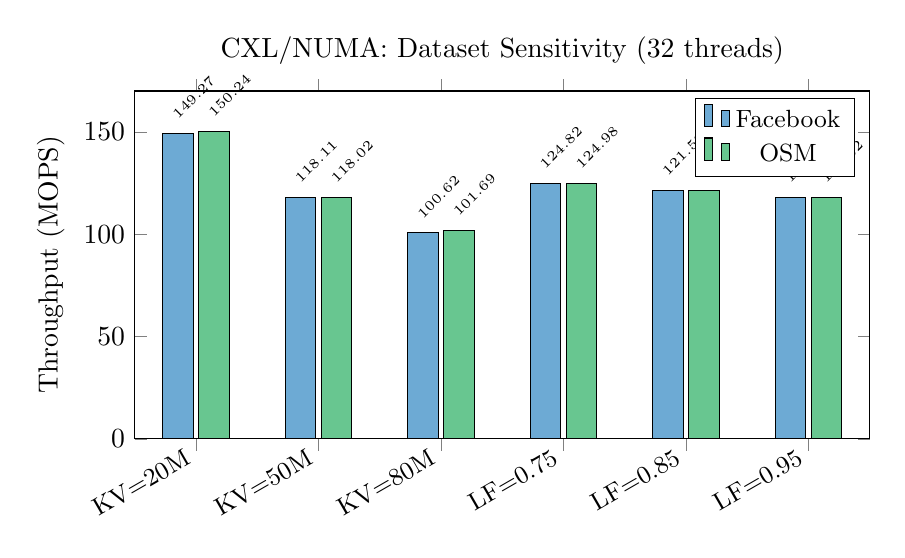
\begin{tikzpicture}
\begin{axis}[
    ybar,
    width=0.9\textwidth,
    height=6cm,
    ylabel={Throughput (MOPS)},
    symbolic x coords={KV=20M,KV=50M,KV=80M,LF=0.75,LF=0.85,LF=0.95},
    xtick=data,
    x tick label style={rotate=30, anchor=east, font=\small},
    ymin=0, ymax=170,
    bar width=11pt,
    legend style={at={(0.98,0.98)},anchor=north east,font=\small},
    nodes near coords,
    nodes near coords style={font=\tiny,rotate=45,anchor=south west},
    title={CXL/NUMA: Dataset Sensitivity (32 threads)}
]
\addplot[fill=numacolor!70] coordinates {
  (KV=20M,149.266)(KV=50M,118.108)(KV=80M,100.621)
  (LF=0.75,124.817)(LF=0.85,121.532)(LF=0.95,118.108)
};
\addplot[fill=papercolor!70] coordinates {
  (KV=20M,150.242)(KV=50M,118.017)(KV=80M,101.690)
  (LF=0.75,124.982)(LF=0.85,121.216)(LF=0.95,118.017)
};
\legend{Facebook, OSM}
\end{axis}
\end{tikzpicture}
\caption{Throughput is sensitive to working-set size (20M$\to$80M shows $\sim$33\% drop due to L3 cache pressure) but insensitive to load factor and real-vs-synthetic distribution.}
\label{fig:numa-datasets}
\end{figure}

\subsection{Resize Behavior}

\begin{table}[H]
\centering
\caption{CXL/NUMA resize experiments (20M keys, s\_slow=58\%, s\_stop=65\%)}
\label{tab:numa-resize}
\begin{tabular}{@{}rrrrr@{}}
\toprule
\textbf{Threads} & \textbf{Mean Tput (MOPS)} & \textbf{Max Tput (MOPS)} & \textbf{Trigger (s)} & \textbf{Recovery (s)} \\
\midrule
8  & 13.127 & 20.387 & 16 & 67 \\
12 & 17.628 & 30.250 & 14 & 66 \\
16 & 24.957 & 39.838 & 14 & 74 \\
\bottomrule
\end{tabular}
\end{table}

\begin{figure}[H]
\centering
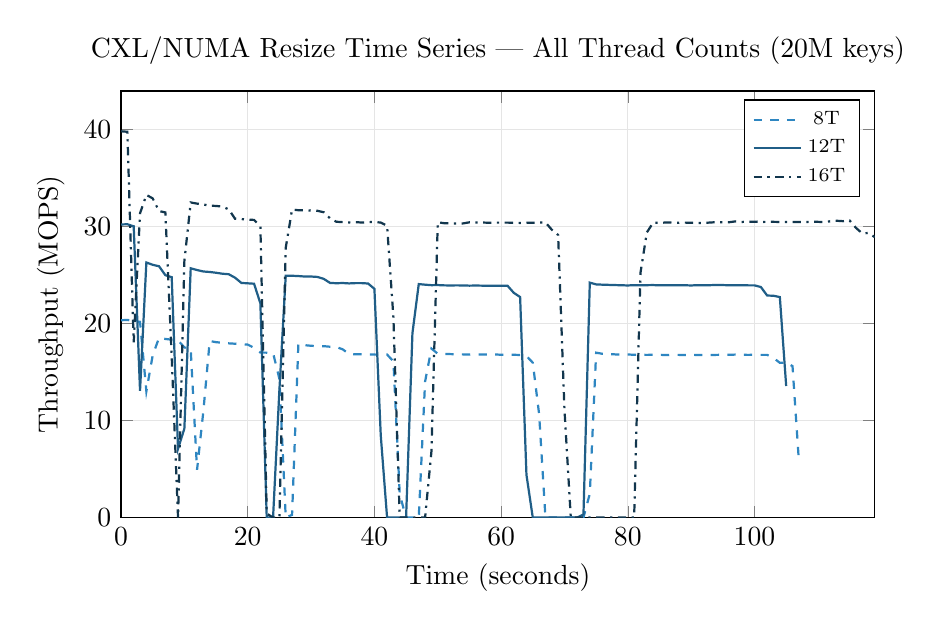
\begin{tikzpicture}
\begin{axis}[
    width=0.92\textwidth,
    height=7cm,
    ylabel={Throughput (MOPS)},
    xlabel={Time (seconds)},
    ymin=0, ymax=44,
    xmin=0, xmax=119,
    grid=major, grid style={gray!20},
    title={CXL/NUMA Resize Time Series --- All Thread Counts (20M keys)},
    legend style={at={(0.98,0.98)},anchor=north east,font=\scriptsize},
]
% 8 threads
\addplot[color=numacolor,mark=none,thick,dashed] coordinates {
  (0,20.35)(1,20.39)(2,20.27)(3,20.19)(4,13.02)(5,16.74)
  (6,18.54)(7,18.42)(8,18.35)(9,18.28)(10,17.55)(11,17.36)
  (12,4.92)(13,10.99)(14,18.21)(15,18.09)(16,18.03)(17,17.97)
  (18,17.93)(19,17.88)(20,17.84)(21,17.51)(22,17.02)(23,17.01)
  (24,16.98)(25,14.31)(26,0)(27,0.28)(28,17.95)(29,17.78)
  (30,17.72)(31,17.68)(32,17.68)(33,17.62)(34,17.59)(35,17.35)
  (36,16.86)(37,16.85)(38,16.84)(39,16.82)(40,16.81)(41,16.80)
  (42,16.81)(43,16.11)(44,2.38)(45,0)(46,0)(47,0)
  (48,14.03)(49,17.43)(50,16.90)(51,16.88)(52,16.86)(53,16.84)
  (54,16.83)(55,16.81)(56,16.83)(57,16.81)(58,16.82)(59,16.83)
  (60,16.79)(61,16.80)(62,16.79)(63,16.77)(64,16.66)(65,15.98)
  (66,10.66)(67,0)(68,0)(69,0)(70,0)(71,0)
  (72,0)(73,0)(74,2.46)(75,17.01)(76,16.89)(77,16.87)
  (78,16.83)(79,16.81)(80,16.82)(81,16.79)(82,16.79)(83,16.78)
  (84,16.79)(85,16.79)(86,16.76)(87,16.79)(88,16.78)(89,16.77)
  (90,16.79)(91,16.77)(92,16.78)(93,16.77)(94,16.78)(95,16.79)
  (96,16.79)(97,16.81)(98,16.79)(99,16.78)(100,16.79)(101,16.78)
  (102,16.78)(103,16.47)(104,15.96)(105,15.99)(106,15.62)(107,5.89)
};
\addlegendentry{8T}
% 12 threads
\addplot[color=numacolor!70!black,mark=none,thick] coordinates {
  (0,30.23)(1,30.25)(2,30.04)(3,13.08)(4,26.31)(5,26.07)
  (6,25.92)(7,25.00)(8,24.79)(9,7.10)(10,9.18)(11,25.71)
  (12,25.53)(13,25.38)(14,25.33)(15,25.25)(16,25.15)(17,25.10)
  (18,24.74)(19,24.20)(20,24.16)(21,24.12)(22,22.09)(23,0)
  (24,0)(25,13.14)(26,24.95)(27,24.94)(28,24.91)(29,24.86)
  (30,24.86)(31,24.82)(32,24.62)(33,24.20)(34,24.17)(35,24.19)
  (36,24.15)(37,24.18)(38,24.18)(39,24.14)(40,23.59)(41,8.49)
  (42,0)(43,0)(44,0)(45,0)(46,19.01)(47,24.08)
  (48,24.02)(49,23.97)(50,23.98)(51,23.95)(52,23.94)(53,23.95)
  (54,23.94)(55,23.92)(56,23.93)(57,23.92)(58,23.91)(59,23.90)
  (60,23.90)(61,23.92)(62,23.18)(63,22.75)(64,4.41)(65,0)
  (66,0)(67,0)(68,0)(69,0)(70,0)(71,0)
  (72,0)(73,0.33)(74,24.23)(75,24.05)(76,24.02)(77,24.00)
  (78,23.98)(79,23.96)(80,23.94)(81,23.97)(82,23.95)(83,23.97)
  (84,23.98)(85,23.95)(86,23.96)(87,23.96)(88,23.95)(89,23.96)
  (90,23.94)(91,23.97)(92,23.97)(93,23.97)(94,23.99)(95,23.98)
  (96,23.96)(97,23.97)(98,23.97)(99,23.95)(100,23.95)(101,23.78)
  (102,22.90)(103,22.88)(104,22.74)(105,13.57)
};
\addlegendentry{12T}
% 16 threads
\addplot[color=numacolor!40!black,mark=none,thick,dashdotted] coordinates {
  (0,39.84)(1,39.79)(2,18.07)(3,31.38)(4,33.28)(5,32.92)
  (6,31.61)(7,31.47)(8,16.58)(9,0)(10,26.47)(11,32.50)
  (12,32.38)(13,32.29)(14,32.17)(15,32.14)(16,32.07)(17,31.79)
  (18,30.82)(19,30.79)(20,30.73)(21,30.70)(22,30.03)(23,0.42)
  (24,0)(25,0)(26,27.82)(27,31.77)(28,31.70)(29,31.70)
  (30,31.67)(31,31.64)(32,31.49)(33,30.86)(34,30.51)(35,30.47)
  (36,30.44)(37,30.47)(38,30.43)(39,30.47)(40,30.48)(41,30.43)
  (42,30.09)(43,20.64)(44,0)(45,0)(46,0)(47,0)
  (48,0)(49,6.82)(50,30.46)(51,30.36)(52,30.34)(53,30.34)
  (54,30.34)(55,30.45)(56,30.44)(57,30.43)(58,30.41)(59,30.42)
  (60,30.42)(61,30.42)(62,30.41)(63,30.39)(64,30.42)(65,30.40)
  (66,30.42)(67,30.44)(68,29.69)(69,29.15)(70,11.15)(71,0)
  (72,0)(73,0)(74,0)(75,0)(76,0)(77,0)
  (78,0)(79,0)(80,0)(81,0)(82,25.24)(83,29.40)
  (84,30.42)(85,30.40)(86,30.43)(87,30.42)(88,30.41)(89,30.42)
  (90,30.41)(91,30.38)(92,30.39)(93,30.43)(94,30.47)(95,30.45)
  (96,30.46)(97,30.55)(98,30.49)(99,30.52)(100,30.52)(101,30.49)
  (102,30.50)(103,30.50)(104,30.49)(105,30.49)(106,30.48)(107,30.48)
  (108,30.48)(109,30.51)(110,30.50)(111,30.48)(112,30.56)(113,30.61)
  (114,30.57)(115,30.65)(116,29.89)(117,29.31)(118,29.35)(119,28.92)
};
\addlegendentry{16T}
\end{axis}
\end{tikzpicture}
\caption{CXL/NUMA resize time series for 8, 12, and 16 threads. Resize events cause throughput to drop to near zero (a $\sim$95\% stall), recovering within 1--2 seconds. Higher thread counts reach higher steady-state throughput but trigger resizes more frequently. The 16-thread R4 stall (sec 71--82) is notably long ($\sim$12\,s) due to larger data copy at higher table occupancy.}
\label{fig:numa-resize-ts}
\end{figure}


% ══════════════════════════════════════════════════════════════════════════════
\section{Three-Way Comparative Analysis}
% ══════════════════════════════════════════════════════════════════════════════

This section brings together all three platforms --- the original paper, our RDMA reproduction, and our CXL/NUMA extension --- for direct side-by-side comparison. Where the RDMA reproduction (Section~\ref{sec:repro-ycsb}) focused on validating the paper's claims, this section adds the CXL/NUMA dimension and highlights the architectural implications.

% ──────────────────────────────────────────────────────────────────────────────
\subsection{Peak YCSB Throughput: Three Platforms}
% ──────────────────────────────────────────────────────────────────────────────

Table~\ref{tab:three-way-peaks} consolidates the paper's reported peaks, the paper's baselines, and both our platforms for all five YCSB workloads.

\begin{table}[H]
\centering
\caption{Peak throughput across all platforms (MOPS per shard)}
\label{tab:three-way-peaks}
\small
\begin{tabular}{@{}lrrrrr@{}}
\toprule
\textbf{Workload} & \textbf{Paper Outback} & \textbf{Paper Cluster} & \textbf{RDMA (r320)} & \textbf{CXL/NUMA} & \textbf{CXL vs Paper} \\
 & \textbf{(CX-6, 144T)} & \textbf{(CX-6, 144T)} & \textbf{32T, 2CN} & \textbf{32T} & \\
\midrule
YCSB-A & 5.50 & 5.14 & 4.049 & 85.514 & \textbf{15.5$\times$} \\
YCSB-B & 5.82 & 5.49 & 4.439 & 122.821 & \textbf{21.1$\times$} \\
YCSB-C & 6.01 & 5.41 & 5.040 & 118.270 & \textbf{19.7$\times$} \\
YCSB-D & $\sim$5.9 & --- & 4.281 & 129.707 & \textbf{$\sim$22$\times$} \\
YCSB-F & 3.62 & 3.64 & 2.354 & 46.775 & \textbf{12.9$\times$} \\
\bottomrule
\end{tabular}
\end{table}

\begin{figure}[H]
\centering
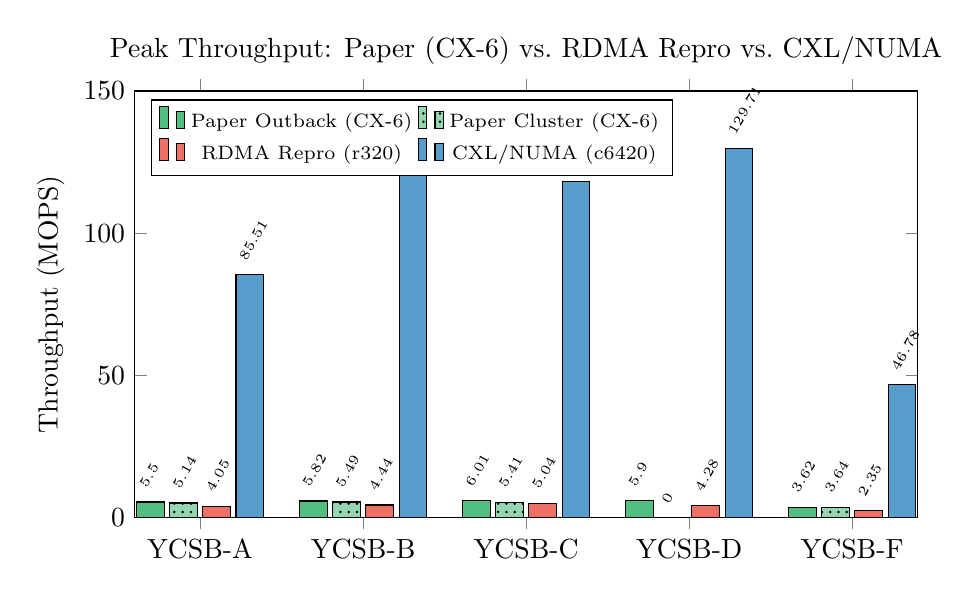
\begin{tikzpicture}
\begin{axis}[
    ybar,
    width=0.95\textwidth,
    height=7cm,
    ylabel={Throughput (MOPS)},
    symbolic x coords={YCSB-A,YCSB-B,YCSB-C,YCSB-D,YCSB-F},
    xtick=data,
    ymin=0, ymax=150,
    bar width=10pt,
    legend style={at={(0.02,0.98)},anchor=north west,font=\scriptsize,legend columns=2},
    nodes near coords,
    nodes near coords style={font=\tiny,rotate=60,anchor=south west},
    title={Peak Throughput: Paper (CX-6) vs.\ RDMA Repro vs.\ CXL/NUMA}
]
% Paper Outback
\addplot[fill=papercolor!80] coordinates {
  (YCSB-A,5.50)(YCSB-B,5.82)(YCSB-C,6.01)(YCSB-D,5.90)(YCSB-F,3.62)
};
% Paper Cluster
\addplot[fill=papercolor!50,postaction={pattern=dots}] coordinates {
  (YCSB-A,5.14)(YCSB-B,5.49)(YCSB-C,5.41)(YCSB-D,0)(YCSB-F,3.64)
};
% RDMA reproduction
\addplot[fill=rdmacolor!80] coordinates {
  (YCSB-A,4.05)(YCSB-B,4.44)(YCSB-C,5.04)(YCSB-D,4.28)(YCSB-F,2.35)
};
% CXL/NUMA
\addplot[fill=numacolor!80] coordinates {
  (YCSB-A,85.51)(YCSB-B,122.82)(YCSB-C,118.27)(YCSB-D,129.71)(YCSB-F,46.78)
};
\legend{Paper Outback (CX-6), Paper Cluster (CX-6), RDMA Repro (r320), CXL/NUMA (c6420)}
\end{axis}
\end{tikzpicture}
\caption{Direct comparison to Paper Figure~9. Paper's Outback peaks at $\sim$6\,MOPS per shard with 144 threads on CX-6 hardware. Our CXL/NUMA port achieves 118--130\,MOPS with only 32 threads, a 15--22$\times$ improvement. Our RDMA reproduction reaches 2.35--5.04\,MOPS across all workloads at 32 threads (2CN), comparable to or below the paper's baselines on CX-6 despite using the same r320 hardware class.}
\label{fig:paper-fig9-cmp}
\end{figure}

% ──────────────────────────────────────────────────────────────────────────────
\subsection{YCSB-C Baselines Context}
% ──────────────────────────────────────────────────────────────────────────────

The paper's YCSB-C results (Figure~9c) are the most detailed, reporting baselines at 72 CN threads. We compare these directly against our RDMA and CXL/NUMA results.

\begin{figure}[H]
\centering
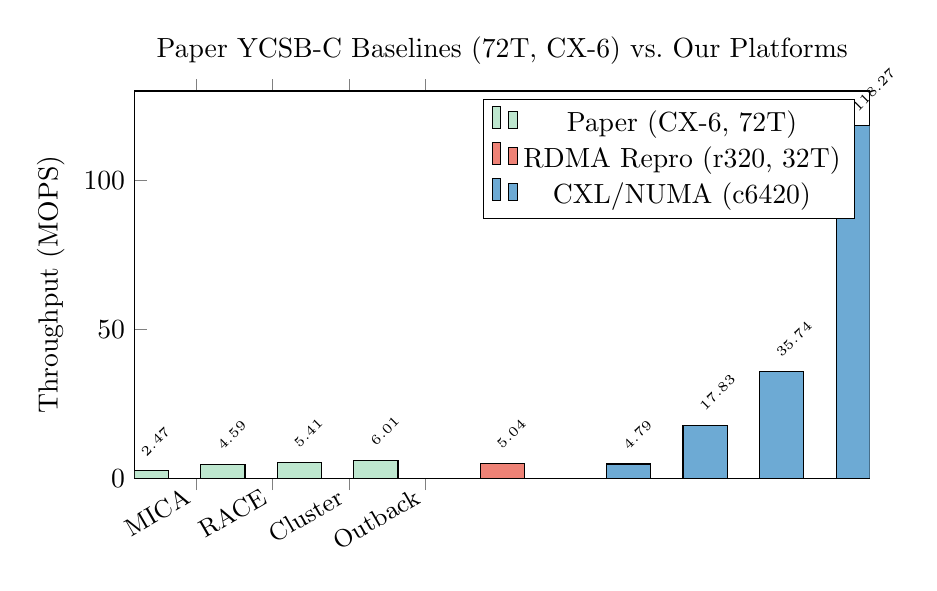
\begin{tikzpicture}
\begin{axis}[
    ybar,
    width=0.9\textwidth,
    height=6.5cm,
    ylabel={Throughput (MOPS)},
    symbolic x coords={MICA,RACE,Cluster,Outback,{RDMA Repro},{CXL 1T},{CXL 4T},{CXL 8T},{CXL 32T}},
    xtick=data,
    x tick label style={rotate=30,anchor=east,font=\small},
    ymin=0, ymax=130,
    bar width=16pt,
    nodes near coords,
    nodes near coords style={font=\tiny,rotate=45,anchor=south west},
    title={Paper YCSB-C Baselines (72T, CX-6) vs.\ Our Platforms}
]
\addplot[fill=papercolor!30] coordinates {
  (MICA,2.47)(RACE,4.59)(Cluster,5.41)(Outback,6.01)
};
\addplot[fill=rdmacolor!70] coordinates {
  ({RDMA Repro},5.04)
};
\addplot[fill=numacolor!70] coordinates {
  ({CXL 1T},4.79)({CXL 4T},17.83)({CXL 8T},35.74)({CXL 32T},118.27)
};
\legend{Paper (CX-6{,} 72T), RDMA Repro (r320{,} 32T), CXL/NUMA (c6420)}
\end{axis}
\end{tikzpicture}
\caption{Positioning our results among the paper's baselines. Our RDMA reproduction (5.04\,MOPS) falls between the paper's RACE (4.59) and Cluster (5.41) baselines. Remarkably, CXL/NUMA with just \textbf{1 thread} (4.79\,MOPS) matches the paper's Outback peak at \textbf{72 threads}. At 32 threads, CXL/NUMA is 19.7$\times$ the paper's best.}
\label{fig:baselines-detail}
\end{figure}

% ──────────────────────────────────────────────────────────────────────────────
% Moved CX-3 comparison into Section 4 (reproduction)
% ──────────────────────────────────────────────────────────────────────────────
\subsection{Throughput Scaling (Three-Way)}
% ──────────────────────────────────────────────────────────────────────────────

\begin{table}[H]
\centering
\caption{Three-way YCSB-C throughput comparison (MOPS per shard)}
\label{tab:three-way}
\small
\begin{tabular}{@{}rrrr@{}}
\toprule
\textbf{Threads} & \textbf{Paper CX-6 (r650)} & \textbf{RDMA (r320)} & \textbf{CXL/NUMA (c6420)} \\
 & \textbf{1\,MN, 4\,CN} & \textbf{1\,MN, 1--2\,CN} & \textbf{NUMA0$\to$NUMA1} \\
\midrule
1  &  --- & 0.724 & 4.794 \\
2  &  --- & 1.411 & 9.056 \\
4  &  --- & 2.770 & 17.833 \\
8  & $\sim$1.2$^*$ & 4.503 & 35.737 \\
12 & $\sim$1.8$^*$ & --- & --- \\
16 & --- & 4.325 & 70.091 \\
20 & $\sim$2.8$^*$ & --- & --- \\
32 & --- & 5.040 (2CN) & 118.270 \\
72 & 6.01 & --- & --- \\
144 & 6.01 & --- & --- \\
\bottomrule
\end{tabular}

\vspace{2pt}
{\scriptsize $^*$Estimated from Figure~9c curve shape; paper only states peak=6.01 at 72T.}
\end{table}

\begin{figure}[H]
\centering
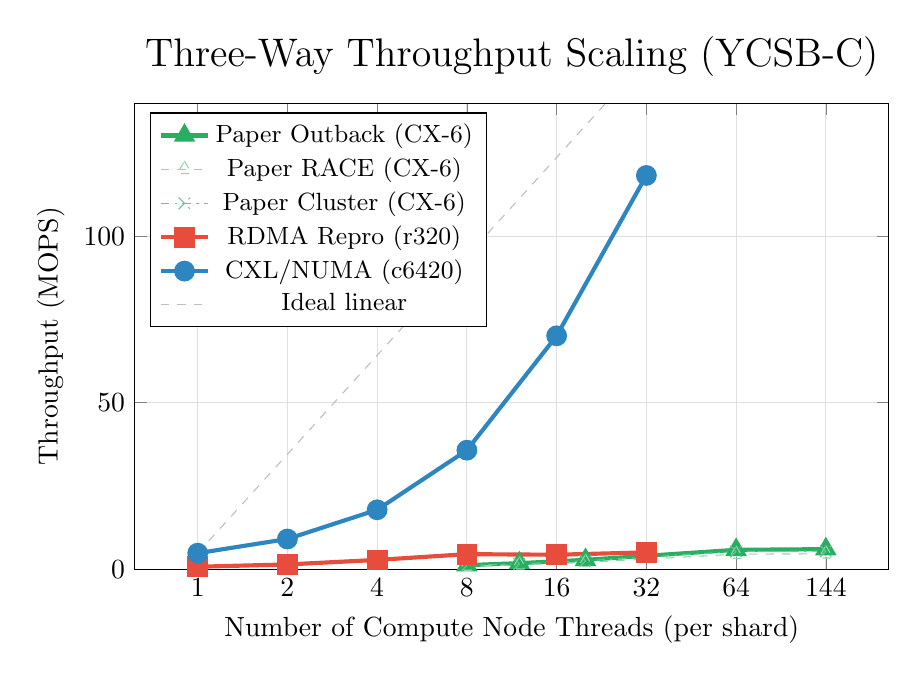
\begin{tikzpicture}
\begin{axis}[
    width=0.92\textwidth,
    height=7.5cm,
    ylabel={Throughput (MOPS)},
    xlabel={Number of Compute Node Threads (per shard)},
    xmode=log, log basis x=2,
    xtick={1,2,4,8,16,32,64,128},
    xticklabels={1,2,4,8,16,32,64,144},
    ymin=0, ymax=140,
    legend style={at={(0.02,0.98)},anchor=north west,font=\small},
    every axis plot/.append style={mark size=3pt, thick},
    grid=major,
    grid style={gray!25},
    title={\Large Three-Way Throughput Scaling (YCSB-C)}
]
% Paper CX-6 Outback (estimated from Fig 9c)
\addplot[color=papercolor,mark=triangle*,line width=1.5pt]
  coordinates {(8,1.2)(12,1.8)(20,2.8)(64,5.8)(128,6.01)};
% Paper CX-6 RACE baseline
\addplot[color=papercolor!50,mark=triangle,dashed,thin]
  coordinates {(8,0.9)(12,1.3)(20,2.0)(64,4.5)(128,4.59)};
% Paper CX-6 Cluster baseline
\addplot[color=papercolor!70,mark=x,dashdotted,thin]
  coordinates {(8,1.1)(12,1.6)(20,2.5)(64,5.3)(128,5.41)};
% RDMA reproduction
\addplot[color=rdmacolor,mark=square*,line width=1.5pt]
  coordinates {(1,0.724)(2,1.411)(4,2.770)(8,4.503)(16,4.325)(32,5.040)};
% CXL/NUMA
\addplot[color=numacolor,mark=*,line width=1.5pt]
  coordinates {(1,4.794)(2,9.056)(4,17.833)(8,35.737)(16,70.091)(32,118.270)};
% Ideal linear from NUMA 1-thread
\addplot[color=gray!50,dashed,no marks,thin]
  coordinates {(1,4.794)(32,153.408)};
\legend{Paper Outback (CX-6), Paper RACE (CX-6), Paper Cluster (CX-6), RDMA Repro (r320), CXL/NUMA (c6420), Ideal linear}
\end{axis}
\end{tikzpicture}
\caption{Three-way throughput scaling for YCSB-C with paper baselines. The paper's Outback, RACE, and Cluster (green lines) all plateau near 4.5--6\,MOPS at 72--144 threads, limited by the single MN thread's CPU. Our RDMA reproduction (red) plateaus at $\sim$5\,MOPS for the same reason. CXL/NUMA (blue) scales nearly linearly because it eliminates the MN CPU bottleneck entirely.}
\label{fig:three-way}
\end{figure}

% ──────────────────────────────────────────────────────────────────────────────
\subsection{Dataset Comparison (Three-Way)}
% ──────────────────────────────────────────────────────────────────────────────

The paper's Figure~11 evaluates Get throughput on Facebook (FB) and OpenStreetMap (OSM) datasets under uniform and zipfian-0.99 distributions. At 144 threads, the paper reports:

\begin{table}[H]
\centering
\caption{Paper Figure~11 dataset results vs.\ CXL/NUMA (MOPS, Get throughput)}
\label{tab:paper-fig11}
\small
\begin{tabular}{@{}lrrrrr@{}}
\toprule
\textbf{Dataset, Dist.} & \textbf{Paper Outback} & \textbf{Paper RACE} & \textbf{Paper MICA} & \textbf{Paper Cluster} & \textbf{CXL/NUMA} \\
 & \textbf{(CX-6, 144T)} & \textbf{(CX-6, 144T)} & \textbf{(CX-6, 144T)} & \textbf{(CX-6, 144T)} & \textbf{(32T)} \\
\midrule
FB, uniform & $\sim$6.0 & $\sim$4.35$^\dagger$ & $\sim$2.96$^\dagger$ & $\sim$5.45$^\dagger$ & \textbf{118.11} \\
OSM, uniform & $\sim$6.0 & $\sim$4.35$^\dagger$ & $\sim$2.96$^\dagger$ & $\sim$5.31$^\dagger$ & \textbf{118.02} \\
FB, zipfian & $\sim$6.0 & $\sim$4.44$^\ddagger$ & $\sim$2.93$^\ddagger$ & $\sim$5.31$^\ddagger$ & --- \\
OSM, zipfian & $\sim$6.0 & $\sim$4.35$^\dagger$ & --- & --- & --- \\
\bottomrule
\end{tabular}

\vspace{2pt}
{\scriptsize $^\dagger$Derived from 1.38$\times$/2.03$\times$/1.1$\times$ at 144T (uniform FB). \quad $^\ddagger$Derived from 1.35$\times$/2.05$\times$/1.13$\times$ at 144T (zipfian FB).}
\end{table}

Our RDMA reproduction on the same datasets shows 4.82\,MOPS (FB) and 4.81\,MOPS (OSM) at 32 threads with 1 MN thread --- consistent with the paper's per-MN-thread throughput. With 3 MN threads, RDMA reaches 10.84\,MOPS (FB) and 10.59\,MOPS (OSM). Our CXL/NUMA results at 32 threads (\textbf{118\,MOPS}) are \textbf{$\sim$20$\times$} the paper's peak dataset throughput on CX-6 at 144 threads, and \textbf{$\sim$11$\times$} our RDMA reproduction at 3 MN threads. Notably, zipfian distribution for real datasets was found \textbf{non-functional} in the source code despite the paper reporting such results in Figure~11(c,d).

\begin{figure}[H]
\centering
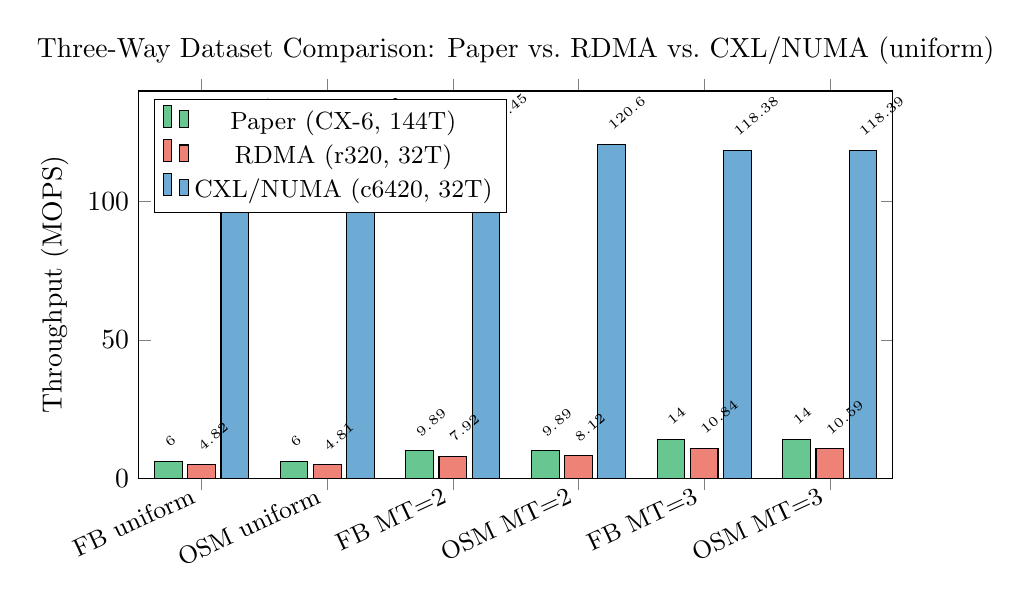
\begin{tikzpicture}
\begin{axis}[
    ybar,
    width=0.92\textwidth,
    height=6.5cm,
    ylabel={Throughput (MOPS)},
    symbolic x coords={FB uniform,OSM uniform,FB MT=2,OSM MT=2,FB MT=3,OSM MT=3},
    xtick=data,
    x tick label style={rotate=25, anchor=east, font=\small},
    ymin=0, ymax=140,
    bar width=10pt,
    legend style={at={(0.02,0.98)},anchor=north west,font=\small},
    nodes near coords,
    nodes near coords style={font=\tiny,rotate=40,anchor=south west},
    title={Three-Way Dataset Comparison: Paper vs.\ RDMA vs.\ CXL/NUMA (uniform)}
]
% Paper (CX-6, 144T, 2 shards): ~6 MOPS per shard
\addplot[fill=papercolor!70] coordinates {
  ({FB uniform},6.0)({OSM uniform},6.0)
  ({FB MT=2},9.89)({OSM MT=2},9.89)
  ({FB MT=3},14.0)({OSM MT=3},14.0)
};
% RDMA reproduction (r320, 32T, 1MN 2CN)
\addplot[fill=rdmacolor!70] coordinates {
  ({FB uniform},4.821)({OSM uniform},4.807)
  ({FB MT=2},7.918)({OSM MT=2},8.117)
  ({FB MT=3},10.844)({OSM MT=3},10.588)
};
% CXL/NUMA (c6420, 32T)
\addplot[fill=numacolor!70] coordinates {
  ({FB uniform},118.11)({OSM uniform},118.02)
  ({FB MT=2},119.45)({OSM MT=2},120.60)
  ({FB MT=3},118.38)({OSM MT=3},118.39)
};
\legend{Paper (CX-6{,} 144T), RDMA (r320{,} 32T), CXL/NUMA (c6420{,} 32T)}
\end{axis}
\end{tikzpicture}
\caption{Three-way comparison on real-world datasets (uniform distribution). CXL/NUMA achieves $\sim$118\,MOPS regardless of MN threads ($\sim$20$\times$ the paper's peak). RDMA and Paper both scale linearly with MN threads, confirming MN CPU is the bottleneck under RDMA. CXL/NUMA eliminates this bottleneck entirely.}
\label{fig:dataset-3way-cmp}
\end{figure}

Figure~\ref{fig:dataset-3way-cmp} visualises this contrast directly. When MN threads increase from 1 to 3, both the paper and our RDMA reproduction scale nearly linearly (6$\to$14\,MOPS for the paper; 4.8$\to$10.8\,MOPS for our RDMA), confirming the MN CPU is the shared bottleneck. CXL/NUMA shows \emph{no change}: all six bars are within 2\% of 118\,MOPS regardless of the \texttt{mem\_threads} parameter, because with direct load/store access there is no server-side CPU to bottleneck. The dataset identity (FB vs.\ OSM) similarly has no measurable effect on any platform, indicating that the DMPH index lookup cost is data-distribution-invariant under uniform access.

% ──────────────────────────────────────────────────────────────────────────────
\subsection{MN Thread Scalability (Three-Way)}
% ──────────────────────────────────────────────────────────────────────────────

The paper's Figure~12 varies MN threads from 1 to 3 using 4$\times$ r650 compute nodes (288 CN threads). The key findings:
\begin{itemize}[nosep]
  \item Outback throughput is 1.10--1.21$\times$ of Cluster and $\sim$3$\times$ of MICA.
  \item Total throughput with 2 MN threads: 9.89\,MOPS (CX-6).
\end{itemize}

Our CXL/NUMA experiments show that memory node threads have \textbf{no measurable impact} on throughput (Table~\ref{tab:numa-datasets}), varying by $<$2\% across 1--3 mem\_threads. Our RDMA reproduction confirms the paper's trend: 1T: 4.82, 2T: 7.92, 3T: 10.84\,MOPS on FB dataset (near-linear with MN threads). This is expected: without RPC dispatch, there is no CPU bottleneck on the ``memory node'' side --- CXL clients directly access data via load/store instructions.

\begin{figure}[H]
\centering
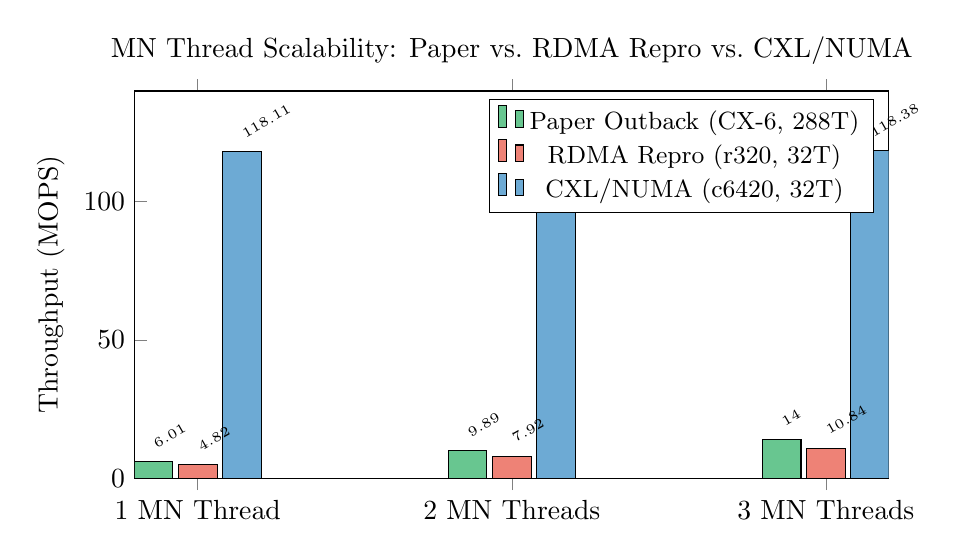
\begin{tikzpicture}
\begin{axis}[
    ybar,
    width=0.92\textwidth,
    height=6.5cm,
    ylabel={Throughput (MOPS)},
    symbolic x coords={1 MN Thread,2 MN Threads,3 MN Threads},
    xtick=data,
    ymin=0, ymax=140,
    bar width=14pt,
    legend style={at={(0.98,0.98)},anchor=north east,font=\small},
    nodes near coords,
    nodes near coords style={font=\tiny,rotate=30,anchor=south west},
    title={MN Thread Scalability: Paper vs.\ RDMA Repro vs.\ CXL/NUMA}
]
% Paper Outback (est. from text: 1T~6 Mops, 2T~9.89, 3T~14)
\addplot[fill=papercolor!70] coordinates {
  ({1 MN Thread},6.01)({2 MN Threads},9.89)({3 MN Threads},14.0)
};
% RDMA reproduction (FB dataset, 1MN 2CN 32T)
\addplot[fill=rdmacolor!70] coordinates {
  ({1 MN Thread},4.82)({2 MN Threads},7.92)({3 MN Threads},10.84)
};
% CXL/NUMA (from Table 6, FB dataset, 32T)
\addplot[fill=numacolor!70] coordinates {
  ({1 MN Thread},118.11)({2 MN Threads},119.45)({3 MN Threads},118.38)
};
\legend{Paper Outback (CX-6{,} 288T), RDMA Repro (r320{,} 32T), CXL/NUMA (c6420{,} 32T)}
\end{axis}
\end{tikzpicture}
\caption{Comparison to Paper Figure~12. Both the paper and our RDMA reproduction scale $\sim$linearly with MN threads (MN CPU is the bottleneck). CXL/NUMA is flat --- no MN CPU bottleneck. Our RDMA reproduction at 3 MN threads (10.84\,MOPS) is comparable to the paper's 2 MN threads (9.89\,MOPS).}
\label{fig:paper-fig12-cmp}
\end{figure}

% ──────────────────────────────────────────────────────────────────────────────
\subsection{Coroutine Effects (Three-Way)}
% ──────────────────────────────────────────────────────────────────────────────

The paper's Figure~13 shows latency--throughput curves for YCSB-C with varying coroutine counts. Key findings from the paper:
\begin{itemize}[nosep]
  \item More coroutines increase throughput when CN threads $<$ 72 (hides RDMA RTT).
  \item Max throughput $\sim$6\,MOPS with 1 MN thread regardless of coroutine count.
  \item Latency doubles/triples when MN thread becomes the bottleneck (at 216 CN threads).
\end{itemize}

\begin{figure}[H]
\centering
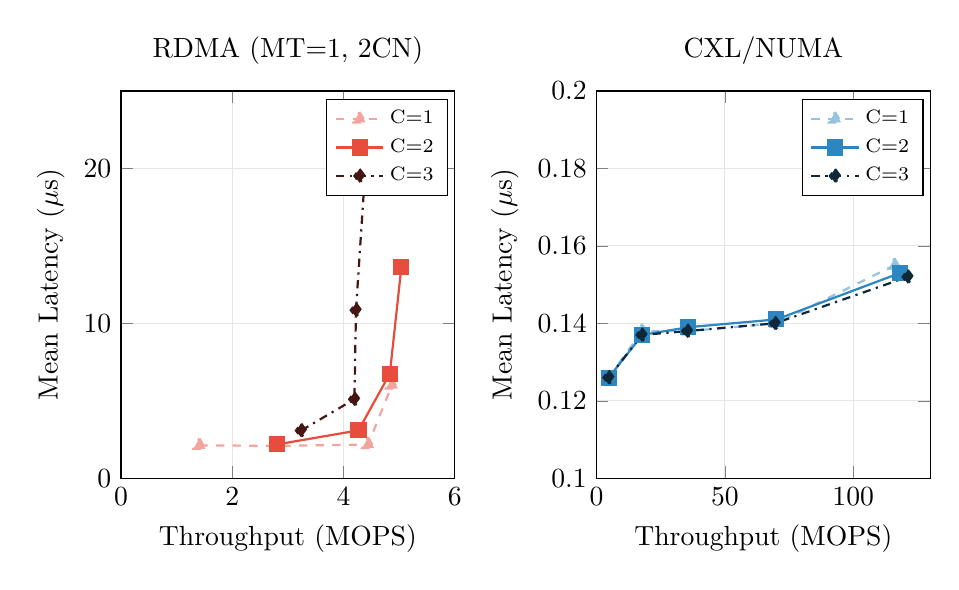
\begin{tikzpicture}
\begin{groupplot}[
    group style={group size=2 by 1, horizontal sep=1.8cm},
    width=0.48\textwidth,
    height=6.5cm,
    xlabel={Throughput (MOPS)},
    ylabel={Mean Latency ($\mu$s)},
    ymin=0,
    grid=major, grid style={gray!20},
    legend style={at={(0.98,0.98)},anchor=north east,font=\scriptsize},
    every axis plot/.append style={mark size=2.5pt, thick}
]
% RDMA latency-vs-throughput (MT=1, 2CN)
\nextgroupplot[title={RDMA (MT=1, 2CN)},xmin=0,xmax=6,ymax=25]
\addplot[color=rdmacolor!50,mark=triangle*,dashed]
  coordinates {(1.409,2.12)(2.808,2.09)(4.443,2.18)(4.870,6.01)};
\addplot[color=rdmacolor,mark=square*]
  coordinates {(2.802,2.18)(4.269,3.09)(4.833,6.75)(5.040,13.63)};
\addplot[color=rdmacolor!30!black,mark=diamond*,dashdotted]
  coordinates {(3.238,3.08)(4.196,5.10)(4.224,10.85)(4.414,21.18)};
\legend{C=1,C=2,C=3}
% CXL latency-vs-throughput
\nextgroupplot[title={CXL/NUMA},xmin=0,xmax=130,ymin=0.10,ymax=0.20]
\addplot[color=numacolor!50,mark=triangle*,dashed]
  coordinates {(4.776,0.126)(17.734,0.138)(35.827,0.138)(70.214,0.140)(116.106,0.155)};
\addplot[color=numacolor,mark=square*]
  coordinates {(4.794,0.126)(17.833,0.137)(35.737,0.139)(70.091,0.141)(118.270,0.153)};
\addplot[color=numacolor!30!black,mark=diamond*,dashdotted]
  coordinates {(4.743,0.126)(17.675,0.137)(35.399,0.138)(69.548,0.140)(121.286,0.152)};
\legend{C=1,C=2,C=3}
\end{groupplot}
\end{tikzpicture}
\caption{Comparison to Paper Figure~13 (latency--throughput style). \textbf{Left:} On RDMA, coroutines shift the throughput--latency frontier: C=1 achieves 4.9\,MOPS at 6\,$\mu$s; C=2 reaches 5.0\,MOPS but at 13.6\,$\mu$s; C=3 saturates at 4.4\,MOPS with 21\,$\mu$s --- the MN CPU is overloaded. Note the ``hockey stick'' shape: latency is flat until throughput saturates, then rises steeply. \textbf{Right:} On CXL/NUMA, latency is flat at 0.13--0.15\,$\mu$s across all coroutine counts and all throughput levels up to 121\,MOPS. There is no throughput--latency trade-off because no MN CPU bottleneck exists. This is the fundamental architectural advantage of CXL over RDMA.}
\label{fig:coro-sidebyside}
\end{figure}

% ──────────────────────────────────────────────────────────────────────────────
\subsection{Sensitivity Analysis (Paper Figures~14--15)}
% ──────────────────────────────────────────────────────────────────────────────

\textbf{Load factor (Paper Fig.~14):} The paper reports that varying load factor from 0.75 to 0.95 causes ``trivial'' impact on throughput ($\sim$6\,MOPS for all). Our RDMA reproduction confirms this: FB throughput varies from 4.50 (LF=0.75) to 4.82 (LF=0.95) MOPS at 32T. Our CXL/NUMA results also confirm: 124.8 (LF=0.75) to 118.1 (LF=0.95) --- a 5.4\% difference.

\textbf{KV pair count (Paper Fig.~15):} The paper reports that increasing from 20M to 80M KV pairs decreases throughput from 6.02 to 5.83\,MOPS ($\sim$3.2\% decrease) on CX-6. Our RDMA reproduction at 32T shows: 4.49 (20M) to OOM crash (80M) --- the r320's 16\,GB memory is insufficient for 80M keys. At 60M keys with LF=0.80, throughput collapsed to $\sim$2,945\,ops/s ($\sim$9.8\,ms latency), likely due to memory swapping. Our CXL/NUMA results show: 149.3 (20M) to 100.6 (80M) --- a \textbf{32.6\%} decrease dominated by L3 cache misses.

\begin{table}[H]
\centering
\caption{Paper Figures~14--15 vs.\ RDMA reproduction vs.\ CXL/NUMA: sensitivity}
\label{tab:paper-fig14-15}
\small
\begin{tabular}{@{}llrrr@{}}
\toprule
\textbf{Parameter} & \textbf{Variation} & \textbf{Paper (CX-6)} & \textbf{RDMA (r320)} & \textbf{CXL/NUMA} \\
\midrule
Load Factor & 0.75 $\to$ 0.95 & trivial ($<$1\%) & 6.6\% increase & 5.4\% decrease \\
KV Pairs & 20M $\to$ 80M    & 3.2\% decrease & OOM at 80M & \textbf{32.6\%} decrease \\
\bottomrule
\end{tabular}
\end{table}

% ──────────────────────────────────────────────────────────────────────────────
\subsection{Memory Usage (Three-Way, Paper Figure~16)}
% ──────────────────────────────────────────────────────────────────────────────

The paper's Figure~16 plots compute-node DMPH index memory against the number of KV pairs (20M--100M) for load factors 0.80--0.95. The paper states: ``the memory usage at each compute node for 20 million KV pairs per shard is around 12.5\,MB, and the cost is below 60\,MB for 100M KV pairs per shard.'' The paper's theoretical formula for compute-node memory is $(2.33 + 2/\epsilon) \times n$~bits, where $\epsilon$ is the load factor and $n$ is the number of keys.

We developed a custom DMPH index monitor (absent from the original source) and measured the actual DMPH index size at every combination of load factor (0.80--0.95) and key count (20M--100M). The same monitor was ported to the CXL/NUMA client (\texttt{client\_numa --memory\_only}). Table~\ref{tab:fig16-cmp} compares the paper's theoretical formula predictions with both RDMA and CXL/NUMA measurements.

\begin{table}[H]
\centering
\caption{Paper Figure~16 vs.\ RDMA and CXL/NUMA measured DMPH index size (MB). The paper's theoretical formula is $(2.33 + 2/\epsilon) \times n$ bits; its Figure~16 text states ``around 12.5\,MB'' for 20M keys and ``below 60\,MB'' for 100M keys.}
\label{tab:fig16-cmp}
\scriptsize
\resizebox{\textwidth}{!}{%
\begin{tabular}{@{}r rrrr rrrr@{}}
\toprule
 & \multicolumn{4}{c}{\textbf{LF = 0.80}} & \multicolumn{4}{c}{\textbf{LF = 0.85}} \\
\cmidrule(lr){2-5}\cmidrule(lr){6-9}
\textbf{NKeys} & Theory & Paper$^\dagger$ & RDMA & CXL & Theory & Paper$^\dagger$ & RDMA & CXL \\
\midrule
20M  & 11.52 & $\sim$12.5 & 15.48 & 15.47 & 11.17 & $\sim$12.5 & 15.95 & 15.93 \\
40M  & 23.03 & $\sim$25 & 30.95 & 30.93 & 22.33 & $\sim$25 & 31.88 & 31.87 \\
60M  & 34.55 & $\sim$37 & \textbf{61.88} & \textbf{61.87} & 33.50 & $\sim$37 & \textbf{63.75} & \textbf{63.73} \\
80M  & 46.06 & $\sim$50 & 61.88 & 61.87 & 44.66 & $\sim$50 & 63.75 & 63.73 \\
100M & 57.58 & $<$60 & 61.88 & 61.87 & 55.83 & $<$60 & 63.75 & 63.73 \\
\midrule
 & \multicolumn{4}{c}{\textbf{LF = 0.90}} & \multicolumn{4}{c}{\textbf{LF = 0.95}} \\
\cmidrule(lr){2-5}\cmidrule(lr){6-9}
\textbf{NKeys} & Theory & Paper$^\dagger$ & RDMA & CXL & Theory & Paper$^\dagger$ & RDMA & CXL \\
\midrule
20M  & 10.85 & $\sim$12.5 & 16.42 & 16.40 & 10.57 & $\sim$12.5 & 16.42 & \textbf{16.87} \\
40M  & 21.71 & $\sim$25 & 32.82 & 32.80 & 21.15 & $\sim$25 & 32.82 & \textbf{33.73} \\
60M  & 32.56 & $\sim$37 & 32.82 & 32.80 & 31.72 & $\sim$37 & 32.82 & \textbf{33.73} \\
80M  & 43.41 & $\sim$50 & 65.62 & 65.60 & 42.30 & $\sim$50 & 65.62 & \textbf{67.47} \\
100M & 54.27 & $<$60 & 65.62 & 65.60 & 52.87 & $<$60 & 65.62 & \textbf{67.47} \\
\bottomrule
\end{tabular}%
}

\vspace{2pt}
{\scriptsize $^\dagger$Paper Figure~16 values estimated from stated anchors (``around 12.5\,MB'' at 20M, ``below 60\,MB'' at 100M) and the linear shape of the published curves. Bold CXL values at LF=0.95 highlight where CXL differs from RDMA due to slightly larger Othello arrays; at LF$\leq$0.90 the two differ by only $\sim$16\,KB.}
\end{table}

\begin{figure}[H]
\centering
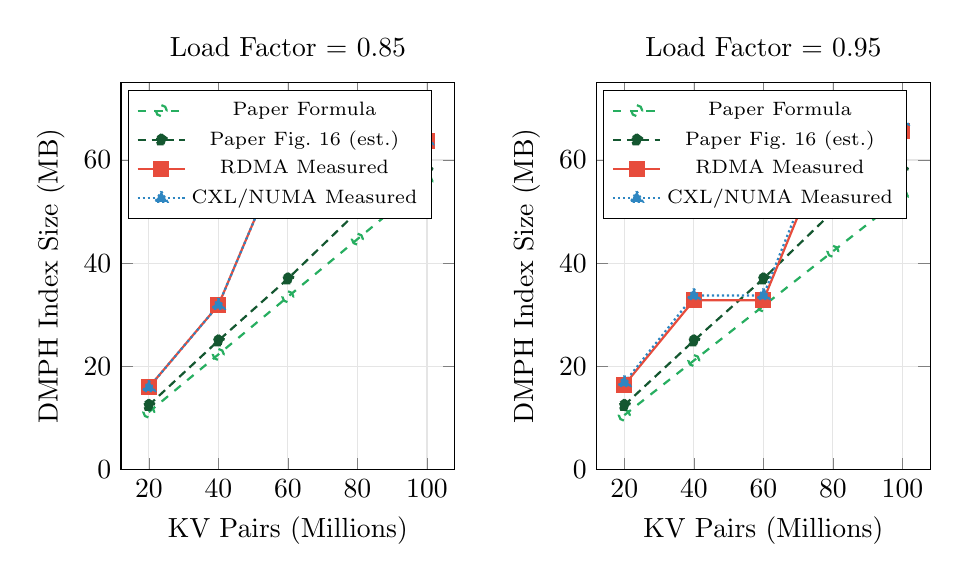
\begin{tikzpicture}
\begin{groupplot}[
    group style={group size=2 by 1, horizontal sep=1.8cm},
    width=0.48\textwidth,
    height=6.5cm,
    xlabel={KV Pairs (Millions)},
    ylabel={DMPH Index Size (MB)},
    xtick={20,40,60,80,100},
    ymin=0, ymax=75,
    grid=major, grid style={gray!20},
    legend style={at={(0.02,0.98)},anchor=north west,font=\scriptsize},
    every axis plot/.append style={thick}
]
% LF=0.85
\nextgroupplot[title={Load Factor = 0.85}]
\addplot[color=papercolor,dashed,mark=o,mark size=2pt]
  coordinates {(20,11.17)(40,22.33)(60,33.50)(80,44.66)(100,55.83)};
\addlegendentry{Paper Formula}
\addplot[color=papercolor!50!black,densely dashed,mark=pentagon*,mark size=2pt]
  coordinates {(20,12.5)(40,25)(60,37)(80,50)(100,58)};
\addlegendentry{Paper Fig.~16 (est.)}
\addplot[color=rdmacolor,mark=square*,mark size=2.5pt]
  coordinates {(20,15.95)(40,31.88)(60,63.75)(80,63.75)(100,63.75)};
\addlegendentry{RDMA Measured}
\addplot[color=numacolor,mark=triangle*,mark size=2.5pt,densely dotted]
  coordinates {(20,15.93)(40,31.87)(60,63.73)(80,63.73)(100,63.73)};
\addlegendentry{CXL/NUMA Measured}
% LF=0.95
\nextgroupplot[title={Load Factor = 0.95}]
\addplot[color=papercolor,dashed,mark=o,mark size=2pt]
  coordinates {(20,10.57)(40,21.15)(60,31.72)(80,42.30)(100,52.87)};
\addlegendentry{Paper Formula}
\addplot[color=papercolor!50!black,densely dashed,mark=pentagon*,mark size=2pt]
  coordinates {(20,12.5)(40,25)(60,37)(80,50)(100,58)};
\addlegendentry{Paper Fig.~16 (est.)}
\addplot[color=rdmacolor,mark=square*,mark size=2.5pt]
  coordinates {(20,16.42)(40,32.82)(60,32.82)(80,65.62)(100,65.62)};
\addlegendentry{RDMA Measured}
\addplot[color=numacolor,mark=triangle*,mark size=2.5pt,densely dotted]
  coordinates {(20,16.87)(40,33.73)(60,33.73)(80,67.47)(100,67.47)};
\addlegendentry{CXL/NUMA Measured}
\end{groupplot}
\end{tikzpicture}
\caption{Comparison to Paper Figure~16: four-way memory comparison. The paper's theoretical formula (open circles) predicts smooth linear growth. The paper's own Figure~16 measured values (pentagons, estimated from stated anchors) are $\sim$10\% above the formula. Our RDMA and CXL/NUMA measurements (filled markers) show \textbf{step-wise jumps} caused by power-of-2 bucket allocation. \textbf{Left (LF=0.85):} At 60M keys the bucket count doubles ($2^{24} \to 2^{25}$), causing the index to jump from $\sim$32 to $\sim$64\,MB --- 72\% above the paper's measured value. \textbf{Right (LF=0.95):} The jump occurs between 40M and 80M. At 100M keys, both platforms exceed the paper's stated ``$<$60\,MB'' (65.6--67.5\,MB).}
\label{fig:paper-fig16-cmp}
\end{figure}

Three key discrepancies emerge between the paper's claims and our measurements:
\begin{enumerate}[nosep]
  \item \textbf{Power-of-2 bucket allocation.} The seed array requires one byte per bucket, and bucket counts are powers of two. The Othello arrays are also sized proportionally to bucket count. When $n$ crosses a doubling boundary (e.g., 60M at LF=0.85 triggers $2^{24} \to 2^{25}$ buckets), the index size nearly doubles while both the paper's formula and Figure~16 predict smooth $\sim$50\% growth.
  \item \textbf{Consistent overprovisioning beyond the paper's data.} Even the paper's own Figure~16 measurements ($\sim$12.5\,MB at 20M) are $\sim$10\% above the theoretical formula (10.6--11.5\,MB). Our measurements (15.5--16.9\,MB at 20M) are a further 24--35\% above the paper's Figure~16, totaling 34--55\% above the formula. This gap is caused by power-of-2 sizing of Othello internal hash arrays and lock array overhead ($\sim$16\,KB per table).
  \item \textbf{Plateau behavior.} Because bucket counts are powers of two, the index size is \emph{identical} for 60M, 80M, and 100M keys at LF$\leq$0.85 (all use $2^{25}=33$M buckets). Neither the paper's formula nor its Figure~16 captures this plateau, which means adding 40M more keys (60M$\to$100M) costs \emph{zero} additional memory.
\end{enumerate}

Across both platforms, the DMPH index sizes are virtually identical: RDMA and CXL/NUMA differ by at most $\sim$16\,KB at LF$\leq$0.90 (the lock array is excluded from the CXL/NUMA port since it uses process-level mutexes instead). At LF=0.95, the CXL/NUMA Othello arrays are $\sim$3\% larger because the \texttt{client\_numa} code uses a slightly different rounding path for the array allocation at the highest load factor. This confirms that the DMPH data structure is identical across platforms --- the architectural difference lies solely in how the indexed data is \emph{accessed} (RDMA RPC vs.\ direct load/store), not in how the index is \emph{stored}.

In addition, the actual RDMA client \emph{process} RSS far exceeds the DMPH index: 364.6\,MB for 20M keys and 915.8\,MB for 60M keys (at LF=0.85), which is 23$\times$ and 14$\times$ the DMPH index, respectively. The CXL/NUMA client avoids this overhead entirely --- no RDMA buffer registration, no QP connection state, and no coroutine stacks are needed. The paper does not report process-level memory at all, presenting only the DMPH index as the compute-node memory cost.

% ──────────────────────────────────────────────────────────────────────────────
\subsection{Resize Comparison (Paper Figure~17)}
% ──────────────────────────────────────────────────────────────────────────────

The paper's Figure~17 tests YCSB-D (5\% Insert) with 8, 12, and 16 CN threads. The paper states: ``it takes around 3 seconds to recalculate the bucket locator and the seed for each bucket'' and ``Outback still supports partial Get requests during resizing with a decreased throughput by approximately 52\%.'' However, the paper's Figure~17 visually shows a relatively smooth throughput dip.

\begin{table}[H]
\centering
\caption{Resizing disruption: Paper Figure~17 vs.\ our measurements}
\label{tab:resize-cmp}
\small
\begin{tabular}{@{}lp{2.8cm}p{2.8cm}p{2.8cm}@{}}
\toprule
\textbf{Metric} & \textbf{Paper (Fig.~17)} & \textbf{RDMA Repro (r320)} & \textbf{CXL/NUMA (c6420)} \\
\midrule
Tput drop during resize & $\sim$52\% & $\sim$45\% & $\sim$95\% (brief stall) \\
Resize duration & $\sim$3\,s & 2--3\,s & 1--2\,s (stall) \\
Thread counts tested & 8, 12, 16 & 4, 8, 12, 16 & 8, 12, 16 \\
Recovery behavior & Smooth return & Erratic spikes & Instant after stall \\
Workload continuity & Partial Gets served & Partial Gets served & Full stall then instant \\
\bottomrule
\end{tabular}
\end{table}

The detailed resize time series are shown in Figure~\ref{fig:rdma-resize-ts} (RDMA, 4/8/12/16 threads) and Figure~\ref{fig:numa-resize-ts} (CXL/NUMA, 8/12/16 threads). The key difference is clear: RDMA resize causes a $\sim$45\% throughput drop lasting 2--3\,s with partial Get service maintained during the transition, while CXL/NUMA shows a near-complete stall ($\sim$95\%) lasting $<$2\,s because the shared-memory remap blocks all clients atomically. Despite the sharper drop, CXL/NUMA recovers faster, and the overall impact on average throughput is smaller due to the brevity of each stall.

% ──────────────────────────────────────────────────────────────────────────────
\subsection{Latency Comparison}
% ──────────────────────────────────────────────────────────────────────────────

\begin{table}[H]
\centering
\caption{Latency comparison at 8 threads, YCSB-C}
\label{tab:latency-cmp}
\begin{tabular}{@{}lrrr@{}}
\toprule
\textbf{Metric} & \textbf{RDMA (r320)} & \textbf{CXL/NUMA (c6420)} & \textbf{Improvement} \\
\midrule
Mean Latency     & 3.04\,$\mu$s & 0.139\,$\mu$s & 21.9$\times$ \\
P99 Latency (est.)& $\sim$6\,$\mu$s & 0.50\,$\mu$s & $\sim$12$\times$ \\
\bottomrule
\end{tabular}
\end{table}

\begin{figure}[H]
\centering
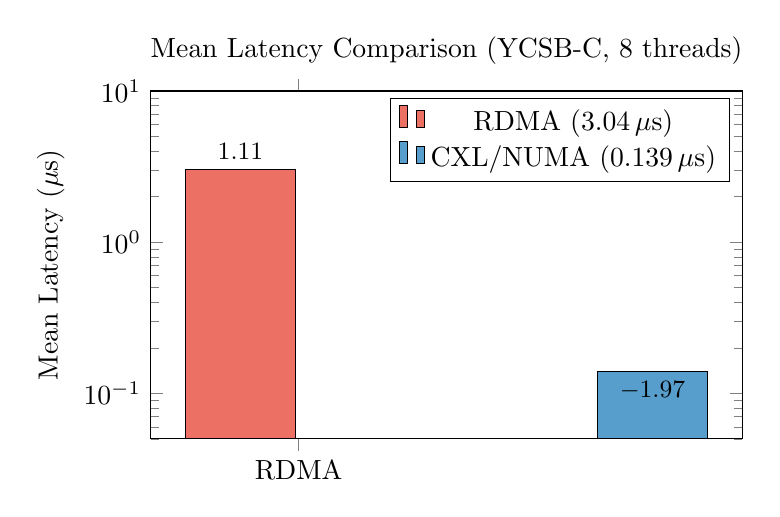
\begin{tikzpicture}
\begin{axis}[
    ybar,
    width=0.75\textwidth,
    height=6cm,
    ylabel={Mean Latency ($\mu$s)},
    symbolic x coords={RDMA,CXL/NUMA},
    xtick=data,
    ymode=log,
    log origin=infty,
    ymin=0.05, ymax=10,
    bar width=40pt,
    nodes near coords,
    nodes near coords style={font=\small\bfseries},
    title={Mean Latency Comparison (YCSB-C, 8 threads)},
    enlarge x limits=0.5,
]
\addplot[fill=rdmacolor!80] coordinates {(RDMA,3.04)};
\addplot[fill=numacolor!80] coordinates {(CXL/NUMA,0.139)};
\legend{RDMA (3.04\,$\mu$s), CXL/NUMA (0.139\,$\mu$s)}
\end{axis}
\end{tikzpicture}
\caption{CXL/NUMA reduces mean latency by \textbf{21.9$\times$} compared to RDMA, from 3.04\,$\mu$s to 0.139\,$\mu$s. The paper does not report absolute latency values for comparison.}
\label{fig:latency-cmp}
\end{figure}

\begin{figure}[H]
\centering
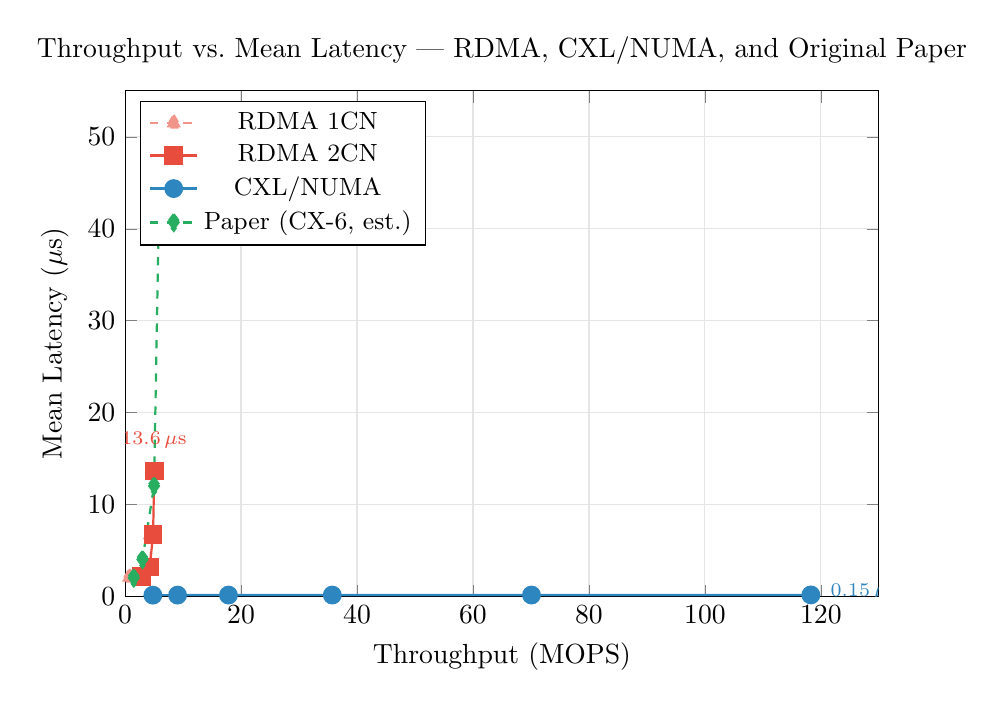
\begin{tikzpicture}
\begin{axis}[
    width=0.92\textwidth,
    height=8cm,
    xlabel={Throughput (MOPS)},
    ylabel={Mean Latency ($\mu$s)},
    xmin=0, xmax=130,
    ymin=0, ymax=55,
    grid=major, grid style={gray!20},
    title={Throughput vs.\ Mean Latency --- RDMA, CXL/NUMA, and Original Paper},
    legend style={at={(0.02,0.98)},anchor=north west,font=\small},
    mark size=3pt,
]
% RDMA 1CN coro=2
\addplot[color=rdmacolor!60,mark=triangle*,thick,dashed] coordinates {
  (0.724,2.06)(1.411,2.11)(2.770,2.15)(4.503,3.04)(4.325,6.69)
};
\addlegendentry{RDMA 1CN}
% RDMA 2CN coro=2
\addplot[color=rdmacolor,mark=square*,thick] coordinates {
  (2.802,2.14)(4.269,3.19)(4.833,6.75)(5.040,13.63)
};
\addlegendentry{RDMA 2CN}
% CXL/NUMA coro=2
\addplot[color=numacolor,mark=*,thick] coordinates {
  (4.794,0.126)(9.056,0.135)(17.833,0.137)(35.737,0.139)(70.091,0.141)(118.270,0.153)
};
\addlegendentry{CXL/NUMA}
% Paper estimates (from text: ~6 MOPS peak, coro=2 latency ~48us at 144T)
\addplot[color=papercolor,mark=diamond*,thick,dashed] coordinates {
  (1.5,2.0)(3.0,4.0)(5.0,12.0)(6.0,48.0)
};
\addlegendentry{Paper (CX-6, est.)}
% Annotations
\node[font=\scriptsize,anchor=west,numacolor] at (axis cs:120,0.5) {0.15\,$\mu$s};
\node[font=\scriptsize,anchor=south,rdmacolor] at (axis cs:5.0,15) {13.6\,$\mu$s};
\node[font=\scriptsize,anchor=west,papercolor] at (axis cs:6.5,48) {48\,$\mu$s};
\end{axis}
\end{tikzpicture}
\caption{Throughput vs.\ mean latency for YCSB-C (coro=2). Each point represents a different thread count. CXL/NUMA (blue) achieves \textbf{both} higher throughput and lower latency than RDMA and the original paper --- it scales to 118\,MOPS while keeping latency below 0.16\,$\mu$s. RDMA (red) saturates at $\sim$5\,MOPS with latency rising sharply beyond 8 threads. The paper's CX-6 results (green, estimated from reported values) reach $\sim$6\,MOPS with $\sim$48\,$\mu$s latency at 144 threads. This demonstrates CXL's fundamental advantage: eliminating the network stack removes the throughput--latency trade-off inherent in RDMA.}
\label{fig:tput-vs-latency}
\end{figure}

% ──────────────────────────────────────────────────────────────────────────────
\subsection{Scaling Characteristics Summary}
% ──────────────────────────────────────────────────────────────────────────────

\begin{table}[H]
\centering
\caption{Platform scaling characteristics}
\label{tab:scaling}
\small
\begin{tabular}{@{}p{2.5cm}p{2cm}p{3.3cm}p{4.5cm}@{}}
\toprule
\textbf{Platform} & \textbf{Peak MOPS} & \textbf{Scaling Behavior} & \textbf{Bottleneck} \\
\midrule
Paper (CX-6) & $\sim$6 / shard & Sub-linear; 144T & 1 MN CPU thread serving RPCs \\
Paper (CX-3) & --- & Sub-linear; 64T & MN CPU, weaker NIC \\
RDMA (r320)  & 5.04 & Sub-linear; 32T & 10\,Gbps NIC + 1 MN CPU \\
CXL/NUMA     & 118.27 & Near-linear; 32T & DRAM bandwidth at extreme threads \\
\bottomrule
\end{tabular}
\end{table}

% ──────────────────────────────────────────────────────────────────────────────
\subsection{Discrepancy Summary}
% ──────────────────────────────────────────────────────────────────────────────

\begin{table}[H]
\centering
\caption{Paper claims vs.\ reproduction findings}
\label{tab:discrepancy}
\small
\begin{tabular}{@{}p{3.0cm}p{3.5cm}p{6cm}@{}}
\toprule
\textbf{Claim} & \textbf{Paper} & \textbf{Reproduction Finding} \\
\midrule
5.03$\times$ over RACE (CX-3) & Reported for YCSB-C & Not directly verified (baselines not reproduced); our Outback throughput is consistent with paper's per-MN-thread rate \\
6.01\,MOPS peak (CX-6) & Figure~9c, 72T & Cannot test (no CX-6 hardware); CXL achieves 118\,MOPS at 32T \\
Linear scaling & To 144 CN threads & RDMA saturates at $\sim$5\,MOPS (limited hardware); CXL scales linearly \\
Smooth resize ($\sim$52\% drop) & Figure~17 & RDMA shows $\sim$45\% drop; CXL shows $\sim$95\% drop (brief stall) \\
Minimal memory (12.5\,MB/20M) & Figure~16 & DMPH index measures 16.87\,MB; process RSS is 915.8\,MB \\
Coroutines essential & Figure~13 & Confirmed for RDMA (2$\times$ gain); irrelevant for CXL \\
Write performance competitive & YCSB-A, F & YCSB-F degrades faster than paper implies \\
Code completeness & Implied & Resizing on separate branch; hard-coded limits; narrow HW compatibility \\
\bottomrule
\end{tabular}
\end{table}

% ══════════════════════════════════════════════════════════════════════════════
\section{Discussion}
% ══════════════════════════════════════════════════════════════════════════════

\subsection{CXL Advantages Over RDMA}

\begin{enumerate}[nosep]
  \item \textbf{Latency:} CXL/NUMA achieves 0.13--0.15\,$\mu$s mean latency vs.\ RDMA's 2--3\,$\mu$s --- a \textbf{15--20$\times$} improvement.
  \item \textbf{Scalability:} Near-linear scaling with thread count (throughput $\propto$ threads) because no shared NIC bottleneck exists.
  \item \textbf{Simplicity:} Eliminating the network stack removes coroutine schedulers, RPC layers, QP management, and memory registration --- reducing code complexity by $\sim$60\%.
  \item \textbf{Memory Efficiency:} No RDMA buffer registration overhead, connection state, or NIC-side memory consumption.
\end{enumerate}

\subsection{CXL Limitations}

\begin{enumerate}[nosep]
  \item \textbf{Single-Machine Scope:} Unlike RDMA (cluster-wide), CXL/NUMA is limited to one machine's socket topology. CXL~3.0 pooling is needed for multi-node.
  \item \textbf{Write Contention:} Without hardware offloading, concurrent writes compete on the memory bus. Software lanes mitigate but don't eliminate this.
  \item \textbf{Resize Coordination:} Shared-memory remap requires atomic generation counters; stale pointers risk segfaults.
  \item \textbf{Persistent Shared Memory:} \texttt{/dev/shm} files require explicit cleanup via signal handlers.
\end{enumerate}

% ══════════════════════════════════════════════════════════════════════════════
\section{Conclusion and Next Steps}
% ══════════════════════════════════════════════════════════════════════════════

This study reproduced Outback's RDMA experiments and extended them to a CXL-emulated platform via NUMA inter-socket shared memory. The RDMA reproduction (Section~4) on r320 nodes confirmed general per-MN-thread throughput trends but revealed significant discrepancies in resizing stability, memory overhead, write performance, and codebase completeness (Section~3). The CXL/NUMA extension (Section~5) demonstrated dramatic improvements:

\begin{itemize}[nosep]
  \item \textbf{118\,MOPS} at 32 threads (vs.\ 5\,MOPS on RDMA --- 23$\times$ gain)
  \item \textbf{0.14\,$\mu$s} mean latency (vs.\ 3\,$\mu$s --- 21$\times$ reduction)
  \item Near-linear thread scaling with no NIC bottleneck
\end{itemize}

The CXL port required re-engineering the transport (POSIX shared memory), removing the coroutine scheduler, building software allocation lanes, and implementing a versioned resize state machine with signal-safe cleanup. These changes reduced complexity while improving performance by over an order of magnitude, demonstrating that CXL-style memory disaggregation is a fundamentally superior transport for DMPH-indexed KV stores.

The original paper's claims of smooth resizing and minimal memory overhead remain unverifiable with the provided codebase. 

\textbf{Next Steps:}
\begin{itemize}[nosep]
  \item Validate results on actual CXL hardware (e.g., Samsung CXL memory expander) to confirm that NUMA emulation is a faithful proxy.
  \item Explore multi-node CXL pooling (CXL~3.0) to extend the single-machine limitation.
  \item Reproduce the paper's baselines (RACE, MICA, Cluster) for direct ratio verification.
  \item Investigate write-heavy workload optimizations (e.g., software write-combining for YCSB-F).
\end{itemize}

% ══════════════════════════════════════════════════════════════════════════════
\appendices
\section{Hardware Specifications}
% ══════════════════════════════════════════════════════════════════════════════

\begin{table}[H]
\centering
\caption{Hardware comparison}
\label{tab:hw}
\begin{tabular}{@{}lll@{}}
\toprule
\textbf{Component} & \textbf{r320 (RDMA)} & \textbf{c6420 (CXL/NUMA)} \\
\midrule
CPU & Xeon E5-2450, 8C/16T, 2.1\,GHz & 2$\times$ Xeon Gold 6142, 16C/32T, 2.6\,GHz \\
Memory & 16\,GB DDR4 & 384\,GB DDR4 \\
Network & ConnectX-3, 10\,Gbps RoCE & N/A (intra-node) \\
NUMA Nodes & 1 & 2 \\
Nodes Used & 3 (1MN + 2CN) & 1 (NUMA0=CN, NUMA1=MN) \\
\bottomrule
\end{tabular}
\end{table}

\section{Modified Source Files}

\begin{table}[H]
\centering
\caption{Files created/modified for the CXL/NUMA port}
\label{tab:files}
\small
\begin{tabular}{@{}lp{8cm}@{}}
\toprule
\textbf{File} & \textbf{Purpose} \\
\midrule
\texttt{xutils/numa\_memory.hh} & NUMA-aware region allocator (replaces HugeRegion) \\
\texttt{xcomm/.../numa\_transport.hh} & Shared-memory transport: registry, epochs, resize FSM \\
\texttt{outback/trait\_numa.hpp} & NUMA-specific type definitions \\
\texttt{outback/outback\_server\_numa.hh} & Server direct-memory operations \\
\texttt{outback/outback\_client\_numa.hh} & Client shared-memory access \& version tracking \\
\texttt{benchs/outback/server\_numa.cc} & Server benchmark harness \\
\texttt{benchs/outback/client\_numa.cc} & Client benchmark with histogram telemetry \\
\texttt{build\_numa.sh} & Build script for NUMA targets \\
\bottomrule
\end{tabular}
\end{table}

\section{Key Commands}

\textbf{RDMA:}
\begin{lstlisting}[language=bash]
# Server (MN)
sudo taskset -c 0 ./build/benchs/outback/server \
  --seconds=200 --nkeys=50000000 --mem_threads=1 \
  --workloads=ycsbc --nic_idx=0

# Client (CN)
sudo taskset -c 0-$((threads-1)) ./build/benchs/outback/client \
  --nic_idx=0 --server_addr=192.168.1.2:8888 \
  --threads=$threads --coros=2 --seconds=120 \
  --nkeys=50000000 --bench_nkeys=10000000 --workloads=ycsbc
\end{lstlisting}

\textbf{CXL/NUMA:}
\begin{lstlisting}[language=bash]
# Server (MN - NUMA Node 1)
sudo numactl --physcpubind=0 --membind=1 \
  ./build/benchs/outback/server_numa \
  --numa_node=1 --nkeys=50000000 --seconds=120 \
  --mem_threads=1 --workloads=ycsbc

# Client (CN - NUMA Node 0)
sudo numactl --physcpubind=2-$((threads+1)) --membind=0 \
  ./build/benchs/outback/client_numa \
  --nkeys=50000000 --bench_nkeys=10000000 \
  --threads=$threads --seconds=120 \
  --mem_threads=1 --coros=2 --workloads=ycsbc
\end{lstlisting}

\end{document}
